%definira klasu dokumenta 
\documentclass[12pt]{report} 

%prostor izmedu naredbi \documentclass i \begin{document} se zove uvod. U njemu se nalaze naredbe koje se odnose na cijeli dokument

%osnovni LaTex ne može riješiti sve probleme, pa se koriste različiti paketi koji olakšavaju izradu željenog dokumenta
\usepackage[croatian]{babel} 
\usepackage{amssymb}
\usepackage{amsmath}
\usepackage{txfonts}
\usepackage{mathdots}
\usepackage{titlesec}
\usepackage{array}
\usepackage{lastpage}
\usepackage{etoolbox}
\usepackage{tabularray}
\usepackage{color, colortbl}
\usepackage{adjustbox}
\usepackage{geometry}
\usepackage[classicReIm]{kpfonts}
\usepackage{hyperref}
\usepackage{fancyhdr}

\usepackage{float}
\usepackage{setspace}
\restylefloat{table}
\graphicspath{ {./slike/} }

\patchcmd{\chapter}{\thispagestyle{plain}}{\thispagestyle{fancy}}{}{} %redefiniranje stila stranice u paketu fancyhdr

%oblik naslova poglavlja
\titleformat{\chapter}{\normalfont\huge\bfseries}{\thechapter.}{20pt}{\Huge}
\titlespacing{\chapter}{0pt}{0pt}{40pt}


\linespread{1.3} %razmak između redaka

\geometry{a4paper, left=1in, top=1in,}  %oblik stranice

\hypersetup{ colorlinks, citecolor=black, filecolor=black, linkcolor=black,	urlcolor=black }   %izgled poveznice


%prored smanjen između redaka u nabrajanjima i popisima
\newenvironment{packed_enum}{
	\begin{enumerate}
		\setlength{\itemsep}{0pt}
		\setlength{\parskip}{0pt}
		\setlength{\parsep}{0pt}
	}{\end{enumerate}}

\newenvironment{packed_item}{
	\begin{itemize}
		\setlength{\itemsep}{0pt}
		\setlength{\parskip}{0pt}
		\setlength{\parsep}{0pt}
	}{\end{itemize}}




%boja za privatni i udaljeni kljuc u tablicama
\definecolor{LightBlue}{rgb}{0.9,0.9,1}
\definecolor{LightGreen}{rgb}{0.9,1,0.9}

%Promjena teksta za dugačke tablice
\DefTblrTemplate{contfoot-text}{normal}{Nastavljeno na idućoj stranici}
\SetTblrTemplate{contfoot-text}{normal}
\DefTblrTemplate{conthead-text}{normal}{(Nastavljeno)}
\SetTblrTemplate{conthead-text}{normal}
\DefTblrTemplate{middlehead,lasthead}{normal}{Nastavljeno od prethodne stranice}
\SetTblrTemplate{middlehead,lasthead}{normal}

%podesavanje zaglavlja i podnožja

\pagestyle{fancy}
\lhead{Programsko inženjerstvo}
\rhead{Company Database}
\lfoot{EkipaZaOcevid}
\cfoot{stranica \thepage/\pageref{LastPage}}
\rfoot{\today}
\renewcommand{\headrulewidth}{0.2pt}
\renewcommand{\footrulewidth}{0.2pt}


\begin{document} 
	
	
	
	\begin{titlepage}
		\begin{center}
			\vspace*{\stretch{1.0}} %u kombinaciji s ostalim \vspace naredbama definira razmak između redaka teksta
			\LARGE Programsko inženjerstvo\\
			\large Ak. god. 2022./2023.\\
			
			\vspace*{\stretch{3.0}}
			
			\huge Company Database\\
			\Large Dokumentacija, Rev. \textit{$<$1 ili 2$>$}\\
			
			\vspace*{\stretch{12.0}}
			\normalsize
			Grupa: \textit{EkipaZaOcevid}\\
			Voditelj: \textit{Petar Hajduk}\\
			
			
			\vspace*{\stretch{1.0}}
			Datum predaje: \textit{$<$dan$>$. $<$mjesec$>$. $<$godina$>$.}\\
	
			\vspace*{\stretch{4.0}}
			
			Nastavnik: \textit{Manuela Lukić}\\
		
		\end{center}

	
	\end{titlepage}

	
	\tableofcontents


	\chapter{Dnevnik promjena dokumentacije}
		
		\textbf{\textit{Kontinuirano osvježavanje}}\\
				
		
		\begin{longtblr}[
				label=none
			]{
				width = \textwidth, 
				colspec={|X[2]|X[13]|X[3]|X[3]|}, 
				rowhead = 1
			}
			\hline
			\textbf{Rev.}	& \textbf{Opis promjene/dodatka} & \textbf{Autori} & \textbf{Datum}\\[3pt] \hline
			0.1 & Napravljen predložak.	& Jakov Jakovac & 22.10.2022. 		\\[3pt] \hline
			0.2 & Napravljeni funkcionalni zahtjevi.	& Marko Čengić & 09.11.2022. 		\\[3pt] \hline
			0.2	& Dopisane upute za povijest dokumentacije.\newline Dodane reference. & * & 24.08.2013. 	\\[3pt] \hline 
			0.5 & Dodan \textit{Use Case} dijagram i jedan sekvencijski dijagram, funkcionalni i nefunkcionalni zahtjevi i dodatak A & * & 25.08.2013. \\[3pt] \hline 
			0.6 & Arhitektura i dizajn sustava, algoritmi i strukture podataka & * & 26.08.2013. \\[3pt] \hline 
			0.8 & Povijest rada i trenutni status implementacije,\newline Zaključci i plan daljnjeg rada & * & 28.08.2013. \\[3pt] \hline 
			0.9 & Opisi obrazaca uporabe & * & 07.09.2013. \\[3pt] \hline 
			0.10 & Preveden uvod & * & 08.09.2013. \\[3pt] \hline 
			0.11 & Sekvencijski dijagrami & * & 09.09.2013. \\[3pt] \hline 
			0.12.1 & Započeo dijagrame razreda & * & 10.09.2013. \\[3pt] \hline 
			0.12.2 & Nastavak dijagrama razreda & * & 11.09.2013. \\[3pt] \hline 
			\textbf{1.0} & Verzija samo s bitnim dijelovima za 1. ciklus & * & 11.09.2013. \\[3pt] \hline 
			1.1 & Uređivanje teksta -- funkcionalni i nefunkcionalni zahtjevi & * \newline * & 14.09.2013. \\[3pt] \hline 
			1.2 & Manje izmjene:Timer - Brojilo vremena & * & 15.09.2013. \\[3pt] \hline 
			1.3 & Popravljeni dijagrami obrazaca uporabe & * & 15.09.2013. \\[3pt] \hline 
			1.5 & Generalna revizija strukture dokumenta & * & 19.09.2013. \\[3pt] \hline 
			1.5.1 & Manja revizija (dijagram razmještaja) & * & 20.09.2013. \\[3pt] \hline 
			\textbf{2.0} & Konačni tekst predloška dokumentacije  & * & 28.09.2013. \\[3pt] \hline 
			&  &  & \\[3pt] \hline	
		\end{longtblr}
	
	
		\textit{Moraju postojati glavne revizije dokumenata 1.0 i 2.0 na kraju prvog i drugog ciklusa. Između tih revizija mogu postojati manje revizije već prema tome kako se dokument bude nadopunjavao. Očekuje se da nakon svake značajnije promjene (dodatka, izmjene, uklanjanja dijelova teksta i popratnih grafičkih sadržaja) dokumenta se to zabilježi kao revizija. Npr., revizije unutar prvog ciklusa će imati oznake 0.1, 0.2, …, 0.9, 0.10, 0.11.. sve do konačne revizije prvog ciklusa 1.0. U drugom ciklusu se nastavlja s revizijama 1.1, 1.2, itd.}
	\chapter{Opis projektnog zadatka}
		
		\textbf{\textit{dio 1. revizije}}\\
		
		\textit{Na osnovi projektnog zadatka detaljno opisati korisničke zahtjeve. Što jasnije opisati cilj projektnog zadatka, razraditi problematiku zadatka, dodati nove aspekte problema i potencijalnih rješenja. Očekuje se minimalno 3, a poželjno 4-5 stranica opisa.	Teme koje treba dodatno razraditi u ovom poglavlju su:}
		\begin{packed_item}
			\item \textit{potencijalna korist ovog projekta}
			\item \textit{postojeća slična rješenja (istražiti i ukratko opisati razlike u odnosu na zadani zadatak). Dodajte slike koja predočavaju slična rješenja.}
			\item \textit{skup korisnika koji bi mogao biti zainteresiran za ostvareno rješenje.}
			\item \textit{mogućnost prilagodbe rješenja }
			\item \textit{opseg projektnog zadatka}
			\item \textit{moguće nadogradnje projektnog zadatka}
		\end{packed_item}
		
		\textit{Za pomoć pogledati reference navedene u poglavlju „Popis literature“, a po potrebi konzultirati sadržaj na internetu koji nudi dobre smjernice u tom pogledu.}
		\eject
		
		\section{Primjeri u \LaTeX u}
		
		\textit{Ovo potpoglavlje izbrisati.}\\

		U nastavku se nalaze različiti primjeri kako koristiti osnovne funkcionalnosti \LaTeX a koje su potrebne za izradu dokumentacije. Za dodatnu pomoć obratiti se asistentu na projektu ili potražiti upute na sljedećim web sjedištima:
		\begin{itemize}
			\item Upute za izradu diplomskog rada u \LaTeX u - \url{https://www.fer.unizg.hr/_download/repository/LaTeX-upute.pdf}
			\item \LaTeX\ projekt - \url{https://www.latex-project.org/help/}
			\item StackExchange za Tex - \url{https://tex.stackexchange.com/}\\
		
		\end{itemize} 	


		
		\noindent \underbar{podcrtani tekst}, \textbf{podebljani tekst}, 	\textit{nagnuti tekst}\\
		\noindent \normalsize primjer \large primjer \Large primjer \LARGE {primjer} \huge {primjer} \Huge primjer \normalsize
				
		\begin{packed_item}
			
			\item  primjer
			\item  primjer
			\item  primjer
			\item[] \begin{packed_enum}
				\item primjer
				\item[] \begin{packed_enum}
					\item[1.a] primjer
					\item[b] primjer
				\end{packed_enum}
				\item primjer
			\end{packed_enum}
			
		\end{packed_item}
		
		\noindent primjer url-a: \url{https://www.fer.unizg.hr/predmet/proinz/projekt}
		
		\noindent posebni znakovi: \# \$ \% \& \{ \} \_ 
		$|$ $<$ $>$ 
		\^{} 
		\~{} 
		$\backslash$ 
		
		
		\begin{longtblr}[
			label=none,
			entry=none
			]{
				width = \textwidth,
				colspec={|X[8,l]|X[8, l]|X[16, l]|}, 
				rowhead = 1,
			} %definicija širine tablice, širine stupaca, poravnanje i broja redaka naslova tablice
			\hline \multicolumn{3}{|c|}{\textbf{naslov unutar tablice}}	 \\ \hline[3pt]
			\SetCell{LightGreen}IDKorisnik & INT	&  	Lorem ipsum dolor sit amet, consectetur adipiscing elit, sed do eiusmod  	\\ \hline
			korisnickoIme	& VARCHAR &   	\\ \hline 
			email & VARCHAR &   \\ \hline 
			ime & VARCHAR	&  		\\ \hline 
			\SetCell{LightBlue} primjer	& VARCHAR &   	\\ \hline 
		\end{longtblr}
		

		\begin{longtblr}[
				caption = {Naslov s referencom izvan tablice},
				entry = {Short Caption},
			]{
				width = \textwidth, 
				colspec = {|X[8,l]|X[8,l]|X[16,l]|}, 
				rowhead = 1,
			}
			\hline
			\SetCell{LightGreen}IDKorisnik & INT	&  	Lorem ipsum dolor sit amet, consectetur adipiscing elit, sed do eiusmod  	\\ \hline
			korisnickoIme	& VARCHAR &   	\\ \hline 
			email & VARCHAR &   \\ \hline 
			ime & VARCHAR	&  		\\ \hline 
			\SetCell{LightBlue} primjer	& VARCHAR &   	\\ \hline 
		\end{longtblr}
	


		
		
		%unos slike
		\begin{figure}[H]
			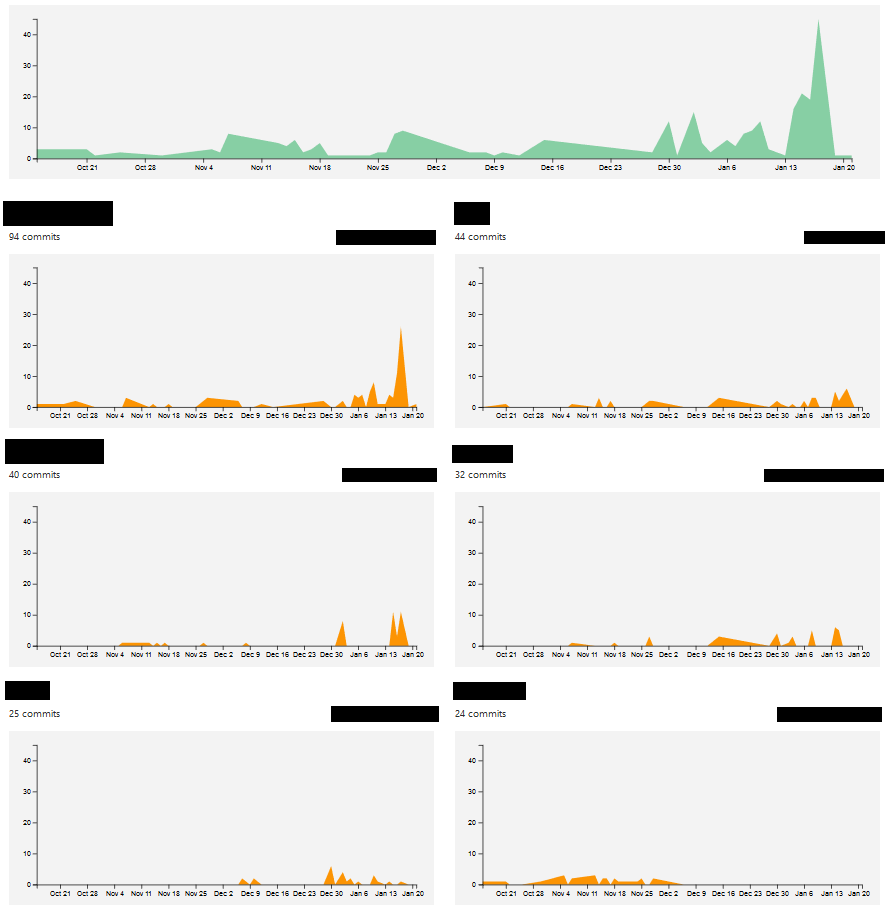
\includegraphics[scale=0.4]{slike/aktivnost.PNG} %veličina slike u odnosu na originalnu datoteku i pozicija slike
			\centering
			\caption{Primjer slike s potpisom}
			\label{fig:promjene}
		\end{figure}
		
		\begin{figure}[H]
			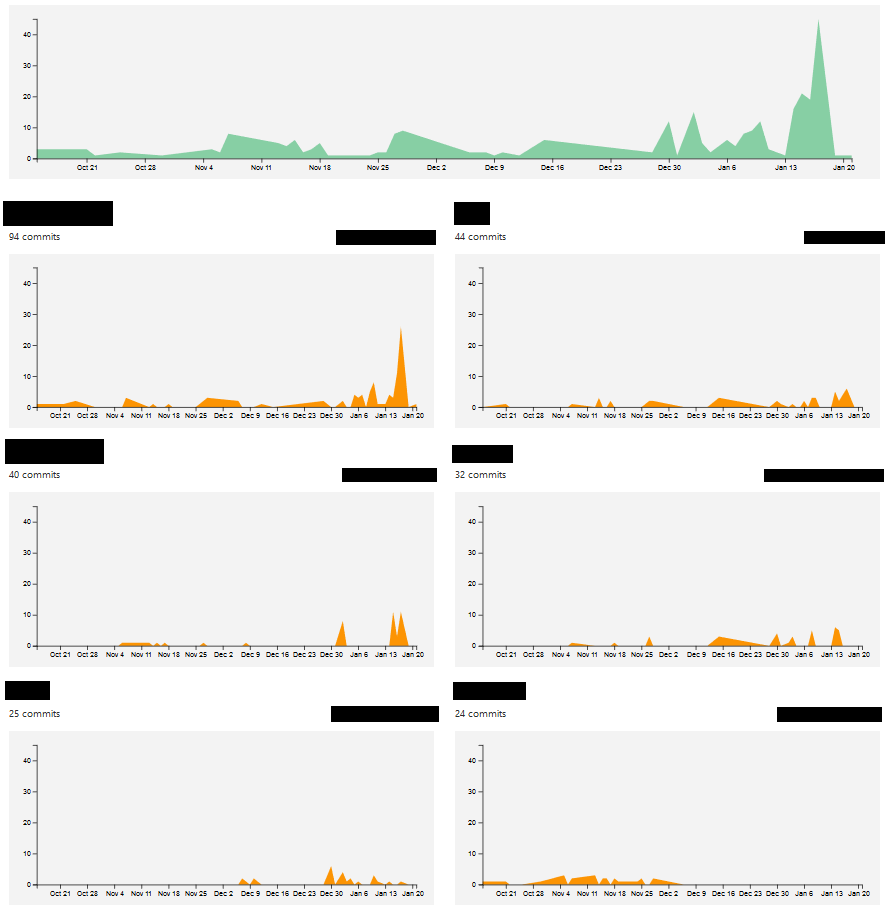
\includegraphics[width=\textwidth]{slike/aktivnost.PNG} %veličina u odnosu na širinu linije
			\caption{Primjer slike s potpisom 2}
			\label{fig:promjene2} %label mora biti drugaciji za svaku sliku
		\end{figure}
		
		Referenciranje slike \ref{fig:promjene2} u tekstu.
		
		\eject
		
	
	\chapter{Specifikacija programske potpore}
		
	\section{Funkcionalni zahtjevi}
			
			\textbf{\textit{dio 1. revizije}}\\

			\textit{Navesti \textbf{dionike} koji imaju \textbf{interes u ovom sustavu} ili \textbf{su nositelji odgovornosti}. To su prije svega korisnici, ali i administratori sustava, naručitelji, razvojni tim.}\\

			\textit{Navesti \textbf{aktore} koji izravno \textbf{koriste} ili \textbf{komuniciraju sa sustavom}. Oni mogu imati inicijatorsku ulogu, tj. započinju određene procese u sustavu ili samo sudioničku ulogu, tj. obavljaju određeni posao. Za svakog aktora navesti funkcionalne zahtjeve koji se na njega odnose.}\\


			\noindent \textbf{Dionici:}
			
			\begin{packed_enum}
				
				\item Predsjednik neprofitabline organizacije
				\item Vlasnik kompanije
				\item Zaposlenik kompanije
					\item Kontakt
					\item Osoba zadužena za prodaju
				\item Član neprofitabline organizacije
					\item Osoba odgovorna za odnose s tvrtkama
					\item Osoba odgovorna za odnose s tvrtkama na projektu
					\item Član tima za odnose s tvrtkama
					\item Intern
				\item Administrator
				\item Razvojni tim
				
			\end{packed_enum}
			
			\noindent \textbf{Aktori i njihovi funkcionalni zahtjevi:}
			
			
			\begin{packed_enum}
				\item  \underbar{Neprijavljeni korisnik (inicijator) moze:}

				\begin{packed_enum}

					\item Ako je nadodan od strane administratora može se prijaviti svojim mailom
					\item U slučaju da je prvi neprijavljeni korisnik postaje administrator

				\end{packed_enum}

				\item  \underbar{Intern -  rola observer (inicijator) može:}
				
				\begin{packed_enum}
					
					\item Pregledavati projekte
					\item Pregledavati kompanije (naziv i područje)
					\item Pregledavati informacija o projektima (datum početka, datum završetka, oganizator)
					\item Pregledavati suradnje
					\item Pregledati korisnike
					\item Pregledati podatke o korisniku
					
				\end{packed_enum}

				\item  \underbar{Član tima za odnose s tvrtkama - rola FR team member (inicijator) može:}

				\begin{packed_enum}

					\item Pregledavati projekte
					\item Pregledavati kompanije (naziv i područje)
					\item Pregledavati informacija o projektima (datum početka, datum završetka, FR- responsiblea)
					\item Pregledavati suradnje
					\item Promijeniti podatke o suradnji (kategorija, status, sažetak, vrijednost)
					\item Pregledavati i promijeniti sve podatke za dodijeljenu kompaniju
					\item Pregledati korisnike
					\item Pregledati podatke o korisniku

				\end{packed_enum}

				\item  \underbar{Osoba odgovorna za odnose s tvrtkama na projektu -  rola FR responsible (inicijator) može:}

				\begin{packed_enum}

					\item Pregledavati projekte
					\item Pregledavati kompanije (naziv i područje)
					\item Pregledavati informacija o projektima (datum početka, datum završetka, FR- responsiblea)
					\item Pregledavati suradnje
					\item Promijeniti podatke o suradnji (kategorija, status, sažetak, vrijednost)
					\item Pregledavati i promijeniti sve podatke za dodijeljenu kompaniju
					\item Strvoriti i obrisati suradnju
					\item Stvoriti i obrisati vlastito stvorene kompanije
					\item Pregledati korisnike
					\item Pregledati podatke o korisniku

				\end{packed_enum}

				\item  \underbar{Osoba odgovorna za odnose s tvrtkama -  rola moderator (inicijator) može:}

				\begin{packed_enum}

					\item Pregledavati projekte
					\item Pregledavati kompanije (naziv i područje)
					\item Pregledavati informacija o projektima (datum početka, datum završetka, FR- responsiblea)
					\item Pregledavati suradnje
					\item Promijeniti podatke o suradnji (kategorija, status, sažetak, vrijednost)
					\item Pregledavati i promijeniti sve podatke za dodijeljenu kompaniju
					\item Strvoriti i obrisati suradnju
					\item Stvoriti i obrisati kompanije
					\item Stvoriti i obrisati vlastito stvorene projekte
					\item Dodijeliti i maknuti nekom korisniku mogućnosti organizatora projekta na projektu koji je stvorio
					\item Staviti i maknuti nekog korisnika s rolom člana neprofitabilne kompanije na projekt koji je stvorio
					\item Pregledati korisnike
					\item Pregledati podatke o korisniku

				\end{packed_enum}

				\item  \underbar{Administrator (inicijator) može:}

				\begin{packed_enum}

					\item Pregledavati projekte
					\item Pregledavati kompanije (naziv i područje)
					\item Pregledavati informacija o projektima (datum početka, datum završetka, FR- responsiblea)
					\item Pregledavati suradnje
					\item Promijeniti podatke o suradnji (kategorija, status, sažetak, vrijednost)
					\item Pregledavati i promijeniti sve podatke za dodijeljenu kompaniju
					\item Strvoriti i obrisati suradnju
					\item Stvoriti i obrisati projekte
					\item Stvoriti i obrisati kompanije
					\item Dodijeliti nekom korisniku mogućnosti organizatora projekta na projektu koji je stvorio
					\item Staviti nekog korisnika s rolom člana neprofitabilne kompanije na projekt koji je stvorio
					\item Pregledati korisnike
					\item Pregledati podatke o korisniku
					\item Dodijeliti nekom korisniku bilo koju od prije navedenih pozicija
					\item Registrirati i maknuti korisnika iz sustava
					\item Registrirati sebe u sustav pri prvom pokretanju
					\item Promijeniti osobne podatake

				\end{packed_enum}
			
				\item  \underbar{Baza podataka (sudionik) može:}
				
				\begin{packed_enum}
					
					\item Pohranjuje sve podatke o projektima
					\item Pohranjuje sve podatke o kompanijama i njihovim kontaktima
					
				\end{packed_enum}

				\item  \underbar{Gmail api (sudionik) može:}

				\begin{packed_enum}

					\item Prijavljuje korisnika pomoću njegovog gmaila

				\end{packed_enum}
			\end{packed_enum}
			
			\eject 
			


			\subsection{Obrasci uporabe}
				
				\textbf{\textit{dio 1. revizije}}
				
				\subsubsection{Opis obrazaca uporabe}
					\textit{Funkcionalne zahtjeve razraditi u obliku obrazaca uporabe. Svaki obrazac je potrebno razraditi prema donjem predlošku. Ukoliko u nekom koraku može doći do odstupanja, potrebno je to odstupanje opisati i po mogućnosti ponuditi rješenje kojim bi se tijek obrasca vratio na osnovni tijek.}

					\noindent \underbar{\textbf{UC1 - Registracija prvog administratora}}
					\begin{packed_item}

						\item \textbf{Glavni sudionik:} Neprijavljeni korisnik
						\item \textbf{Cilj:} Stvoriti administratov korisnički račun za pristup aplikaciji
						\item \textbf{Sudionici:} Baza podataka, Google auth API
						\item \textbf{Preduvjet:} - 
						\item \textbf{Opis osnovnog tijeka:}

						\item[] \begin{packed_enum}

							\item Korisnik dolazi na stranicu koja ga preusmjerava na formu za registraciju prvog korisnika
							\item Korisnik ispunjava formu emailom prvog administratora
							\item Stranica preusmjerava korisnika na osnovnu stranicu

						\end{packed_enum}

						\item \textbf{Opis mogućih odstupanja:}

						\item[] \begin{packed_item}

							\item[2.a] Upis već postojećeg emaila ili upis korisničkih
							podatka u nedozvoljenom formatu
							\item[] \begin{packed_enum}

								\item Aplikacija obavještava korisnika o neuspjelom upisu
								\item Administrator mijenja potrebne podatke te uspješno završava unos ili
								odustaje od dodavanja novog korisnika

							\end{packed_enum}

						\end{packed_item}
					\end{packed_item}

					\noindent \underbar{\textbf{UC2 - Prijava u aplikaciju}}
					\begin{packed_item}
	
						\item \textbf{Glavni sudionik:} Neprijavljeni korisnik
						\item \textbf{Cilj:} Dati korisniku pristup aplikaciji
						\item \textbf{Sudionici:} Baza podataka
						\item \textbf{Preduvjet:} Korisnik je registriran
						\item \textbf{Opis osnovnog tijeka:}
						
						\item[] \begin{packed_enum}
	
							\item Korisnik dolazi na stranicu za prijavu
							\item Otvara mu se prozor za prijavu s google računom
							\item Korisnik se prijavljuje google računom
							\item Korisnik dobiva pristup aplikaciji koja preusmjava na naslovnu stranicu
						\end{packed_enum}
						
						\item \textbf{Opis mogućih odstupanja:}

						\item[] \begin{packed_item}

							\item[2.a] Prijavom s računom koji nije u bazi
							\item[] \begin{packed_enum}

								\item Aplikacija obavještava korisnika o neuspjeloj prijavi
								\item Aplikacija obavještava korisnika na koju email adresu se treba javiti ako korisnik smatra da je to greška
								\item Korisnik se ponovo prijavljuje s drugim računom ili odustaje od prijave

							\end{packed_enum}

						\end{packed_item}
					\end{packed_item}

					\noindent \underbar{\textbf{UC3 - Registracija korisnika}}
					\begin{packed_item}

						\item \textbf{Glavni sudionik:} Administrator
						\item \textbf{Cilj:} Stvoriti korisnički račun za pristup aplikaciji
						\item \textbf{Sudionici:} Baza podataka
						\item \textbf{Preduvjet:} Korisnik je prijavljen
						\item \textbf{Opis osnovnog tijeka:}

						\item[] \begin{packed_enum}

							\item Korisnik (administrator) odabire opciju "Users"
							\item Aplikacija prikazuje popis korisnika
							\item Korisnik odabire opciju za dodavanje korisnika
							\item Aplikacija prikaže formu za dodavanje korisnika
							\item Korisnik popuni potrebne podatke (ime, prezime, email i razinu ovlasti)
							\item Korisnik odabere opciju "Add"
							\item Baza podataka se ažurira
							\item Aplikacija zatvori formu za dodavanje korisnika
							\item Aplikacija ažurira popis korisnika
						\end{packed_enum}

						\item \textbf{Opis mogućih odstupanja:}

						\item[] \begin{packed_item}

							\item[3.a] Upis već postojećeg emaila ili upis korisničkih
							podatka u nedozvoljenom formatu
							\item[] \begin{packed_enum}

								\item Aplikacija obavještava korisnika o neuspjelom upisu
								\item Administrator mijenja potrebne podatke te uspješno završava unos ili
								odustaje od dodavanja novog korisnika

							\end{packed_enum}

						\end{packed_item}
					\end{packed_item}

					\noindent \underbar{\textbf{UC4 - Pregled projekata}}
					\begin{packed_item}

						\item \textbf{Glavni sudionik:} Intern
						\item \textbf{Cilj:} Pregledati projekte
						\item \textbf{Sudionici:} Baza podataka
						\item \textbf{Preduvjet:} Korisnik je prijavljen
						\item \textbf{Opis osnovnog tijeka:}

						\item[] \begin{packed_enum}

							\item Korisnik odabire opciju "Projects"
							\item Aplikacija prikazuje popis naziva projekata
						\end{packed_enum}
					\end{packed_item}

					\noindent \underbar{\textbf{UC5 - Pregled kompanija}}
					\begin{packed_item}

						\item \textbf{Glavni sudionik:} Intern
						\item \textbf{Cilj:} Pregledati kompanije
						\item \textbf{Sudionici:} Baza podataka
						\item \textbf{Preduvjet:} Korisnik je prijavljen
						\item \textbf{Opis osnovnog tijeka:}

						\item[] \begin{packed_enum}

							\item Korisnik odabire opciju "Companies"
							\item Aplikacija prikazuje popis kompanijama s osnovnim podacima (naziv, područje, ABC kategorizacija i link na web)
						\end{packed_enum}
					\end{packed_item}

					\noindent \underbar{\textbf{UC6 - Pregled podataka o projektu}}
					\begin{packed_item}

						\item \textbf{Glavni sudionik:} Intern
						\item \textbf{Cilj:} Pregledati podatke o projektu
						\item \textbf{Sudionici:} Baza podataka
						\item \textbf{Preduvjet:} Korisnik je prijavljen
						\item \textbf{Opis osnovnog tijeka:}

						\item[] \begin{packed_enum}

							\item Korisnik odabire opciju "Projects"
							\item Aplikacija prikazuje popis projekata
							\item Korisnik klikne na naziv projekta o kojem želi informacije
							\item Prikažu se detalji projekta
						\end{packed_enum}
					\end{packed_item}

					\noindent \underbar{\textbf{UC7 - Pregled podataka o korisniku}}
					\begin{packed_item}

						\item \textbf{Glavni sudionik:} Intern
						\item \textbf{Cilj:} Pregledati podatke o željenom korisniku
						\item \textbf{Sudionici:} Baza podataka
						\item \textbf{Preduvjet:} Korisnik je prijavljen
						\item \textbf{Opis osnovnog tijeka:}

						\item[] \begin{packed_enum}

							\item Korisnik odabire opciju "Users"
							\item Aplikacija prikazuje popis korisnika
							\item Korisnik odabire željenog korisnika iz popisa
							\item Aplikacija prikazuje podatke o korisniku
						\end{packed_enum}
					\end{packed_item}

					\noindent \underbar{\textbf{UC8 - Promjena podataka o korisniku}}
					\begin{packed_item}

						\item \textbf{Glavni sudionik:} Administrator
						\item \textbf{Cilj:} Promijeniti podatke o korisniku
						\item \textbf{Sudionici:} Baza podataka
						\item \textbf{Preduvjet:} Korisnik je prijavljen, Korisnik ima razinu ovlasti administrator
						\item \textbf{Opis osnovnog tijeka:}

						\item[] \begin{packed_enum}

							\item Korisnik odabire opciju "Users"
							\item Aplikacija prikazuje popis korisnika
							\item Korisnik odabire opciju "Edit"
							\item Aplikacija prikaže formu za izmjenu podataka korisnika
							\item Korisnik mijenja podatke
							\item Korisnik odabire opciju spremi
							\item Baza podataka se ažurira
							\item Aplikacija zatvori formu za dodavanje korisnika
							\item Aplikacija ažurira popis korisnika
						\end{packed_enum}

						\item \textbf{Opis mogućih odstupanja:}

						\item[] \begin{packed_item}

							\item[2.f] Upis već postojećeg emaila ili upis korisničkih
							podatka u nedozvoljenom formatu
							\item[] \begin{packed_enum}

								\item Aplikacija obavještava korisnika o neuspjelom upisu
								\item Administrator mijenja potrebne podatke te uspješno završava unos ili
								odustaje od izmjene podataka o korisniku

							\end{packed_enum}

						\end{packed_item}
					\end{packed_item}

					\noindent \underbar{\textbf{UC9 - Pregled suradnji}}
					\begin{packed_item}
					
						\item \textbf{Glavni sudionik:} Intern
						\item \textbf{Cilj:} Pregledati podatke o suradnji
						\item \textbf{Sudionici:} Baza podataka
						\item \textbf{Preduvjet:} Korisnik je prijavljen, Korisnik je FR team member projekta
						\item \textbf{Opis osnovnog tijeka:}

						\item[] \begin{packed_enum}

							\item Korisnik odabire opciju "Projects"
							\item Aplikacija prikazuje popis projekata
							\item Korisnik klikne na ime projekta u kojem se nalazi suradnja koja ga zanima
							\item Aplikacija prikazuje popis suradnji vezanih uz taj projekt sa osnovnim podacima (naziv kompanije, odgovoru osobu, status, kategoriju, kontakt, dio komentara, akcije)
						\end{packed_enum}
	
					\end{packed_item}

					\noindent \underbar{\textbf{UC10 - Promjena podataka o suradnji}}
					\begin{packed_item}

						\item \textbf{Glavni sudionik:} Član tima za odnose s tvrtkama
						\item \textbf{Cilj:} Promijeniti podatke o suradnji
						\item \textbf{Sudionici:} Baza podataka
						\item \textbf{Preduvjet:} Korisnik je prijavljen, Korisnik je FR reponsible projekta
						\item \textbf{Opis osnovnog tijeka:}

						\item[] \begin{packed_enum}

							\item Korisnik odabire opciju "Projects"
							\item Aplikacija prikazuje popis projekata
							\item Korisnik klikne na ime projekta u kojem se nalazi suradnja koja ga zanima
							\item Aplikacija prikazuje popis suradnji vezanih uz taj projekt sa osnovnim podacima (naziv kompanije, odgovoru osobu, status, kategoriju, kontakt, dio komentara, akcije)
							\item Korisnik odabire opciju "Edit"
							\item Aplikacija prikaže formu s podacima te suradnje
							\item Korisnik mijenja podatke o suradnji
							\item Korisnik odabire opciju "Save"
							\item Baza podataka se ažurira
							\item Aplikacija ažurira popis suradnji

						\end{packed_enum}
						
						\item \textbf{Opis mogućih odstupanja:}

						\item[] \begin{packed_item}

							\item[7.a] Korisnik promijeni podatke o suradnji na nevažeće vrijednosti
							i odabere opciju "Save"
							
							\item[] \begin{packed_enum}

								\item Aplikacija obavještava korisnika o neuspjelom upisu
								\item Administrator mijenja potrebne podatke te uspješno završava unos ili
								odustaje od promjene podataka

							\end{packed_enum}

						\end{packed_item}
						
					\end{packed_item}

					\noindent \underbar{\textbf{UC11 - Pregled podataka o kompaniji}}
					\begin{packed_item}

						\item \textbf{Glavni sudionik:} Član tima za odnose s tvrtkama
						\item \textbf{Cilj:} Pregledati podatke o kompaniji
						\item \textbf{Sudionici:} Baza podataka
						\item \textbf{Preduvjet:} Korisnik je prijavljen, Korisnik ima razinu ovlasti FR responsible
						\item \textbf{Opis osnovnog tijeka:}

						\item[] \begin{packed_enum}

							\item Korisnik odabire opciju "Companies"
							\item Aplikacija prikaže popis kompanija
							\item Korisnik odabire kompaniju
							\item Aplikacija prikaže detalje o toj kompaniji
						\end{packed_enum}
					\end{packed_item}

					\noindent \underbar{\textbf{UC12 - Promjena podataka o kompaniji}}
					\begin{packed_item}

						\item \textbf{Glavni sudionik:} Član tima za odnose s tvrtkama
						\item \textbf{Cilj:} Promijeniti podatke o kompaniji
						\item \textbf{Sudionici:} Baza podataka
						\item \textbf{Preduvjet:} Korisnik je prijavljen, Korisnik je odgovoran za suradnju s kompanijom
						\item \textbf{Opis osnovnog tijeka:}

						\item[] \begin{packed_enum}

							\item Korisnik odabire opciju "Companies"
							\item Aplikacija prikaže popis kompanija
							\item Korisnik odabire kompaniju za koju je dodijeljen
							\item Aplikacija prikaže podatke o kompaniji
							\item Korisnik odabire opciju "Edit"
							\item Aplikacija prikaže formu s podacima o kompaniji
							\item Korisnik mijenja podatke o kompaniji
							\item Korisnik sprema promjene
							\item Baza podataka se ažurira
							\item Aplikacija zatvori formu s podacima o kompaniji
							\item Aplikacija ažurira podatke o kompaniji
						\end{packed_enum}

						\item \textbf{Opis mogućih odstupanja:}

						\item[] \begin{packed_item}

							\item[5.b] Korisnik promijeni podatke o kompaniji na nevaljane podatke i odabere opciju "Save"
							\item[] \begin{packed_enum}

								\item Aplikacija obavještava korisnika o neuspjelom upisu
								\item Korisnik mijenja potrebne podatke te uspješno završava unos ili
								odustaje od promjene podataka

							\end{packed_enum}

						\end{packed_item}
					\end{packed_item}

					\noindent \underbar{\textbf{UC13 - Stvaranje suradnje za dodijeljen projekt}}
					\begin{packed_item}

						\item \textbf{Glavni sudionik:} Osoba odgovorna za odnose s tvrtkama na projektu
						\item \textbf{Cilj:} Stvoriti suradnju za dodijeljen projekt
						\item \textbf{Sudionici:} Baza podataka
						\item \textbf{Preduvjet:} Korisnik je prijavljen
						\item \textbf{Opis osnovnog tijeka:}

						\item[] \begin{packed_enum}

							\item Korisnik odabire opciju "Projects"
							\item Aplikacija prikazuje popis projekata
							\item Korisnik klikne na ime projekta u kojem želi stvoriti suradnju
							\item Aplikacija prikazuje popis suradnji vezanih uz taj projekt sa osnovnim podacima (naziv kompanije, odgovoru osobu, status, kategoriju, kontakt, dio komentara, akcije)
							\item Korisnik odabere opciju "New collaboration"
							\item Aplikacija prikaže formu za stvaranje nove suradnje
							\item Korisnik popunjava podatke o suradnji
							\item Korisnik sprema promjene
							\item Baza podataka se ažurira
							\item Aplikacija zatvara formu za stvaranje nove suradnje
							\item Aplikacija ažurira popis suradnji
						\end{packed_enum}

						\item \textbf{Opis mogućih odstupanja:}

						\item[] \begin{packed_item}

							\item[8.c] Korisnik unese nevaljane podatke o suradnji i odabere opciju "Save"
							\item[] \begin{packed_enum}

								\item Aplikacija obavještava korisnika o neuspjelom upisu
								\item Korisnik mijenja potrebne podatke te uspješno završava unos ili
								odustaje od dodavanja suradnje

							\end{packed_enum}

						\end{packed_item}
					\end{packed_item}

					\noindent \underbar{\textbf{UC14 - Brisanje suradnje}}
					\begin{packed_item}

						\item \textbf{Glavni sudionik:} Osoba odgovorna za odnose s tvrtkama na projektu
						\item \textbf{Cilj:} Maknuti suradnju sa dodijeljenog projekta
						\item \textbf{Sudionici:} Baza podataka
						\item \textbf{Preduvjet:} Korisnik je prijavljen
						\item \textbf{Opis osnovnog tijeka:}

						\item[] \begin{packed_enum}

							\item Korisnik odabire opciju "Projects"
							\item Aplikacija prikazuje popis projekata
							\item Korisnik klikne na ime projekta u kojem se nalazi suradnja koja ga zanima
							\item Aplikacija prikazuje popis suradnji vezanih uz taj projekt sa osnovnim podacima (naziv kompanije, odgovoru osobu, status, kategoriju, kontakt, dio komentara, akcije)
                            \item Korisnik odabere opciju za brisanje suradnje
                            \item Aplikacija pita korisnika je li siguran želi li izbrisati suradnju
                            \item Korisnik odabire potvrdnu opciju
                            \item Baza podataka se ažurira
                            \item Aplikacija ažurira popis suradnji
                            
						\end{packed_enum}
					\end{packed_item}

					\noindent \underbar{\textbf{UC15 - Stvaranje projekta}}
					\begin{packed_item}

						\item \textbf{Glavni sudionik:} Osoba odgovorna za odnose s tvrtkama
						\item \textbf{Cilj:} Stvoriti projekt
						\item \textbf{Sudionici:} Baza podataka
						\item \textbf{Preduvjet:} Korisnik je prijavljen
						\item \textbf{Opis osnovnog tijeka:}

						\item[] \begin{packed_enum}

							\item Korisnik odabire opciju "Projects"
							\item Aplikacija prikazuje popis projekata
							\item Korisnik odabire opciju "Create project"
							\item Aplikacija prikazuje formu za stvaranje novog projekta
							\item Korisnik popuni podatke za stvaranje novog projekta
							\item Korisnik sprema promjene
							\item Baza podataka se ažurira
							\item Aplikacija ažurira popis projekata
						\end{packed_enum}

						\item \textbf{Opis mogućih odstupanja:}

						\item[] \begin{packed_item}

							\item[7.b] Korisnik unese nevaljane podatke o projektu i odabere opciju "Save"
							\item[] \begin{packed_enum}

								\item Aplikacija obavještava korisnika o neuspjelom upisu
								\item Korisnik mijenja potrebne podatke te uspješno završava unos ili
								odustaje od dodavanja projekta

							\end{packed_enum}

						\end{packed_item}
					\end{packed_item}

					\noindent \underbar{\textbf{UC16 - Brisanje projekta}}
					\begin{packed_item}
					
						\item \textbf{Glavni sudionik:} Osoba odgovorna za odnose s tvrtkama
						\item \textbf{Cilj:} Izbrisati projekt
						\item \textbf{Sudionici:} Baza podataka
						\item \textbf{Preduvjet:} Korisnik je prijavljen
						\item \textbf{Opis osnovnog tijeka:}
					
						\item[] \begin{packed_enum}

							\item Korisnik odabire opciju "Projects"
							\item Aplikacija prikazuje popis projekata
							\item Korisnik odabire neki od projekata
							\item Aplikacija prikazuje detalje o tom projektu
							\item Korisnik odabire opciju za brisanje projekta
							\item Aplikacija prikaže modal koji pita korisnika je li siguran
							\item Korisnik odabere opciju da je siguran
							\item Baza podataka se ažurira
							\item Aplikacija ažurira popis projekata
						\end{packed_enum}
					
					\end{packed_item}

					\noindent \underbar{\textbf{UC17 - Dodavanje korisnika na projekt}}
					\begin{packed_item}

						\item \textbf{Glavni sudionik:} Osoba odgovorna za odnose s tvrtkama
						\item \textbf{Cilj:} Dodati člana neprofitabilne organizacije na projekt
						\item \textbf{Sudionici:} Baza podataka
						\item \textbf{Preduvjet:} Korisnik je prijavljen
						\item \textbf{Opis osnovnog tijeka:}
					
						\item[] \begin{packed_enum}
					
							\item Korisnik odabire opciju "Projects"
							\item Aplikacija prikazuje popis projekata
							\item Korisnik odabire neki od projekata
							\item Aplikacija prikazuje detalje o tom projektu
							\item Korisnik odabire opciju za dodavanje korisnika na projekt
							\item Aplikacija prikaže formu
							\item Korisnik upiše ime, prezime, nadimak ili email člana kojeg želi dodati
							\item Korisnik odabire opciju "Add"
							\item Baza podataka se ažurira
							\item Aplikacija ažurira popis korisnika na projektu
						\end{packed_enum}
					
						\item \textbf{Opis mogućih odstupanja:}
					
						\item[] \begin{packed_item}
                        
                        	\item[7.b] Korisnik unese nevaljane podatke o korisniku i odabere opciju "Add"
							\item[] \begin{packed_enum}

								\item Aplikacija obavještava korisnika o neuspjelom upisu
								\item Korisnik mijenja potrebne podatke te uspješno završava unos ili
								odustaje od dodavanja korisnika na projekt

							\end{packed_enum}
					
						\end{packed_item}
					\end{packed_item}

					\noindent \underbar{\textbf{UC18 - Micanje korisnika sa projekta}}
					\begin{packed_item}

						\item \textbf{Glavni sudionik:} Osoba odgovorna za odnose s tvrtkama
						\item \textbf{Cilj:} Maknuti člana neprofitabilne organizacije sa projekt
						\item \textbf{Sudionici:} Baza podataka
						\item \textbf{Preduvjet:} Korisnik je prijavljen
						\item \textbf{Opis osnovnog tijeka:}

						\item[] \begin{packed_enum}

							\item Korisnik odabire opciju "Projects"
							\item Aplikacija prikazuje popis projekata
							\item Korisnik odabire neki od projekata
							\item Aplikacija prikazuje detalje o tom projektu
							\item Korisnik odabire opciju za micanje korisnika sa projekta
							\item Aplikacija prikaže modal koji pita korisnika je li siguran
							\item Korisnik odabere opciju da je siguran
							\item Baza podataka se ažurira
							\item Aplikacija ažurira popis korisnika na projektu
						\end{packed_enum}

					\end{packed_item}

					\noindent \underbar{\textbf{UC19 - Pregled korisnika}}
					\begin{packed_item}

						\item \textbf{Glavni sudionik:} Intern
						\item \textbf{Cilj:} Pregledati korisnike
						\item \textbf{Sudionici:} Baza podataka
						\item \textbf{Preduvjet:} Korisnik je prijavljen
						\item \textbf{Opis osnovnog tijeka:}

						\item[] \begin{packed_enum}

							\item Korisnik odabire opciju "Users"
							\item Aplikacija prikazuje popis korisnika
                            
						\end{packed_enum}
					\end{packed_item}

					\noindent \underbar{\textbf{UC20 - Promjena razine ovlasti korisnika}}
					\begin{packed_item}

						\item \textbf{Glavni sudionik:} Administrator
						\item \textbf{Cilj:} Promijeniti rolu korisnika
						\item \textbf{Sudionici:} Baza podataka
						\item \textbf{Preduvjet:} Korisnik je prijavljen
						\item \textbf{Opis osnovnog tijeka:}

						\item[] \begin{packed_enum}

							\item Korisnik odabire opciju "Users"
							\item Aplikacija prikazuje popis korisnika
							\item Korisnik odabere opciju za izmjenu podataka o korisniku
							\item Aplikacija prikaže formu za izmjenu podataka o korisniku
							\item Korisnik odabire jednu od razina ovlasti
							\item Korisnik odabire opciju spremi
							\item Baza podataka se ažurira
							\item Aplikacija ažurira popis korisnika

						\end{packed_enum}

						\item \textbf{Opis mogućih odstupanja:}

						\item[] \begin{packed_item}

							\item[3.a] Korisnik kojem se mijenja rola je administrator i ne postoji nijedan
							drugi administrator
							\item[] \begin{packed_enum}

								\item Sustav obavještava korisnika da mora postojati
								barem jedan administrator, pa je ova akcija zabranjena

							\end{packed_enum}

						\end{packed_item}
					\end{packed_item}

					\noindent \underbar{\textbf{UC21 - Brisanje korisnika iz sustava}}
					\begin{packed_item}

						\item \textbf{Glavni sudionik:} Administrator
						\item \textbf{Cilj:} Maknuti korisnika iz sustava
						\item \textbf{Sudionici:} Baza podataka
						\item \textbf{Preduvjet:} Korisnik je prijavljen
						\item \textbf{Opis osnovnog tijeka:}

						\item[] \begin{packed_enum}

							\item Korisnik odabire opciju "Users"
							\item Aplikacija prikazuje popis korisnika
							\item Korisnik odabere opciju brisanja željenog korisnika
							\item Aplikacija pita korisnika je li siguran da želi provesti ovu akciju
							\item Korisnik odabire opciju da je siguran
							\item Baza podataka se ažurira
							\item Aplikacija ažurira popis korisnika

						\end{packed_enum}

						\item \textbf{Opis mogućih odstupanja:}

						\item[] \begin{packed_item}

							\item[3.a] Korisnik kojem se miče iz sustava je administrator i ne postoji nijedan
							drugi administrator
							\item[] \begin{packed_enum}

								\item Sustav obavještava korisnika da mora postojati
								barem jedan administrator, pa je ova akcija zabranjena

							\end{packed_enum}

						\end{packed_item}
					\end{packed_item}

					\noindent \underbar{\textbf{UC22 - Filtriranje korisnika}}
					\begin{packed_item}

						\item \textbf{Glavni sudionik:} Intern
						\item \textbf{Cilj:} Filtrirati korisnike
						\item \textbf{Sudionici:} Baza podataka
						\item \textbf{Preduvjet:} Korisnik je prijavljen
						\item \textbf{Opis osnovnog tijeka:}

						\item[] \begin{packed_enum}

							\item Korisnik odabire opciju "Users"
							\item Aplikacija prikazuje popis korisnika
							\item Korisnik upiše tekst u polje za pretragu
							\item Aplikacija ažurira popis korisnika tako da prikazuje samo korisnike koji imaju taj tekst u imenu, prezimenu, nadimku ili emailu
						\end{packed_enum}
					\end{packed_item}

					\noindent \underbar{\textbf{UC23 - Stvaranje kompanije}}
					\begin{packed_item}

						\item \textbf{Glavni sudionik:} Osoba odgovorna za odnose s tvrtkama na projektu
						\item \textbf{Cilj:} Stvoriti kompaniju
						\item \textbf{Sudionici:} Baza podataka
						\item \textbf{Preduvjet:} Korisnik je prijavljen
						\item \textbf{Opis osnovnog tijeka:}

						\item[] \begin{packed_enum}

							\item Korisnik odabire opciju "Companies"
							\item Aplikacija prikazuje popis kompanija
							\item Korisnik odabire opciju "Create company"
							\item Aplikacija prikazuje formu za stvaranje nove kompanije
							\item Korisnik popuni podatke za stvaranje nove kompanije
							\item Korisnik sprema promjene
							\item Baza podataka se ažurira
							\item Aplikacija ažurira popis kompanija

						\end{packed_enum}

						\item \textbf{Opis mogućih odstupanja:}

						\item[] \begin{packed_item}

							\item[7.b] Korisnik unese nevaljane podatke o kompaniji i odabere opciju "Save"
							\item[] \begin{packed_enum}

								\item Aplikacija obavještava korisnika o neuspjelom upisu
								\item Korisnik mijenja potrebne podatke te uspješno završava unos ili
								odustaje od dodavanja kompanije

							\end{packed_enum}

						\end{packed_item}
					\end{packed_item}

					\noindent \underbar{\textbf{UC24 - Brisanje kompanije}}
					\begin{packed_item}

						\item \textbf{Glavni sudionik:} Osoba odgovorna za odnose s tvrtkama na projektu
						\item \textbf{Cilj:} Izbrisati kompaniju
						\item \textbf{Sudionici:} Baza podataka
						\item \textbf{Preduvjet:} Korisnik je prijavljen
						\item \textbf{Opis osnovnog tijeka:}

						\item[] \begin{packed_enum}

							\item Korisnik odabire opciju "Companies"
							\item Aplikacija prikazuje popis kompanija
							\item Korisnik odabire gumb za detalje pored neke od kompanija
							\item Aplikacija prikazuje detalje o toj kompaniji
							\item Korisnik odabire opciju za brisanje kompanije
							\item Aplikacija prikaže modal koji pita korisnika je li siguran
							\item Korisnik odabere opciju da je siguran
							\item Baza podataka se ažurira
							\item Aplikacija ažurira popis projekata

						\end{packed_enum}

					\end{packed_item}
					
				\subsubsection{Dijagrami obrazaca uporabe}

					\begin{figure}[H]
						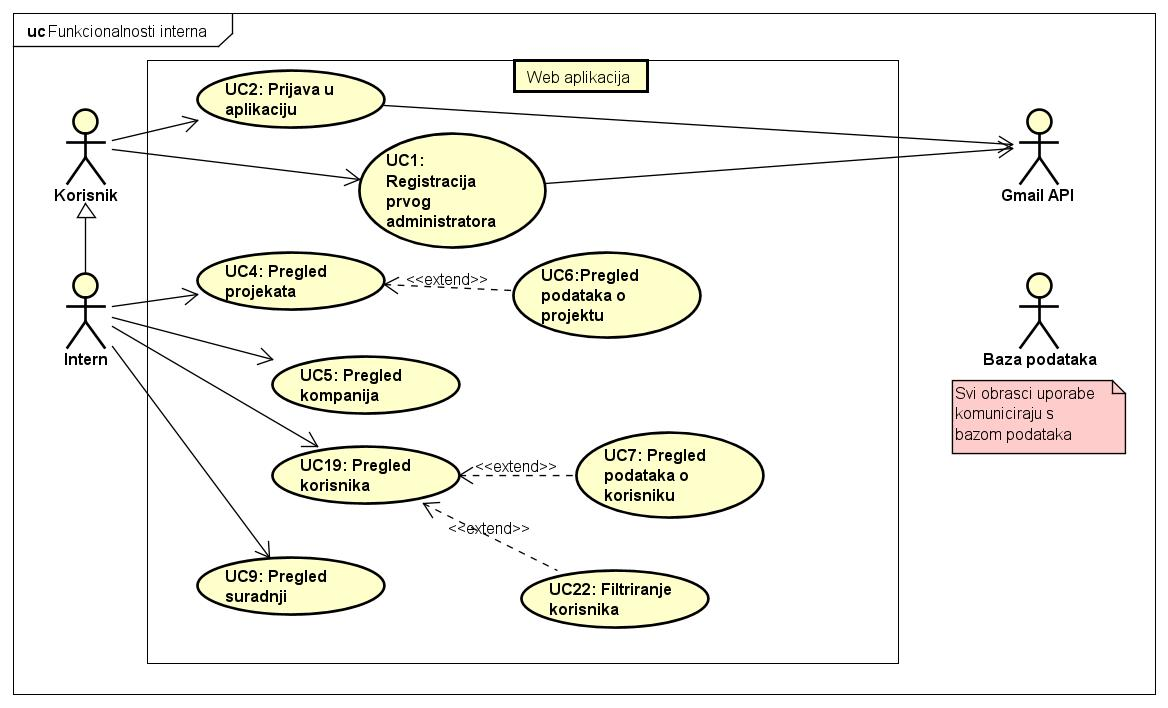
\includegraphics[scale=0.4]{slike/UC dijagrami/UseCase observer}
						\centering
						\caption{Slika 3.1: Dijagram obrasca uporabe, funkcionalnosti interna i korisnika}
						\label{fig:observer}
					\end{figure}

					\begin{figure}[H]
						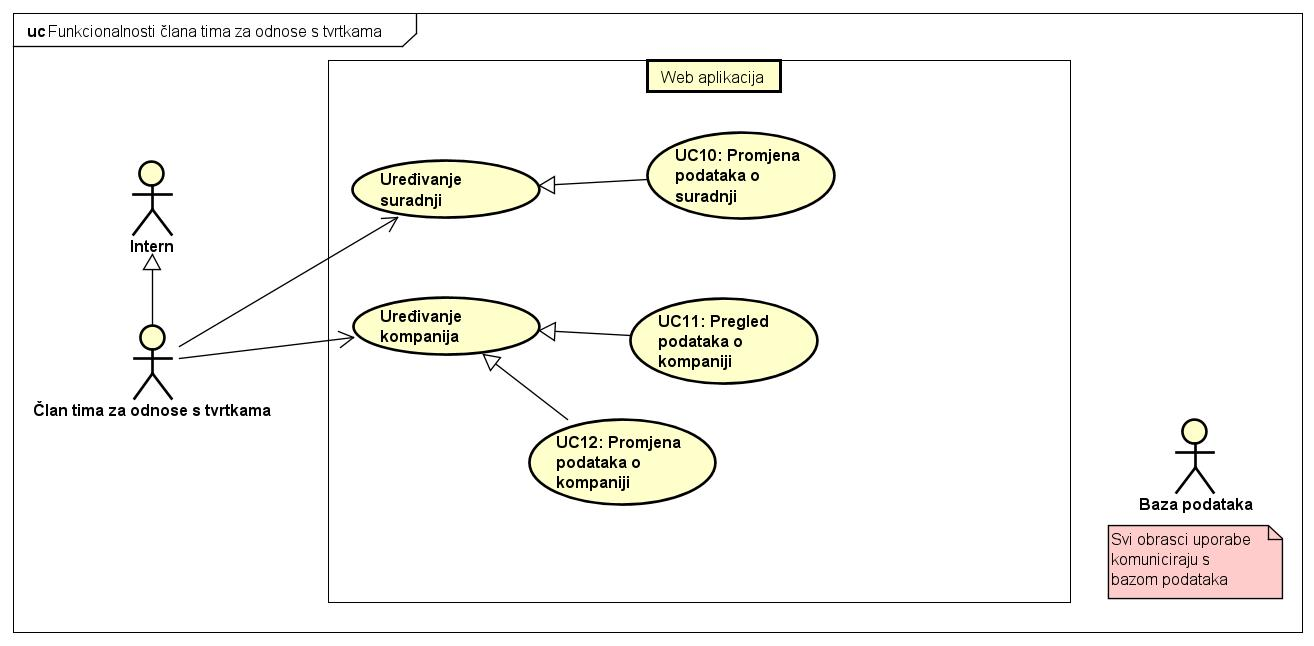
\includegraphics[scale=0.4]{slike/UC dijagrami/UseCase FR team member}
						\centering
						\caption{Slika 3.2: Dijagram obrasca uporabe, funkcionalnosti člana tima za odnose s tvrtkama}
						\label{fig:frTeamMember}
					\end{figure}

					\begin{figure}[H]
						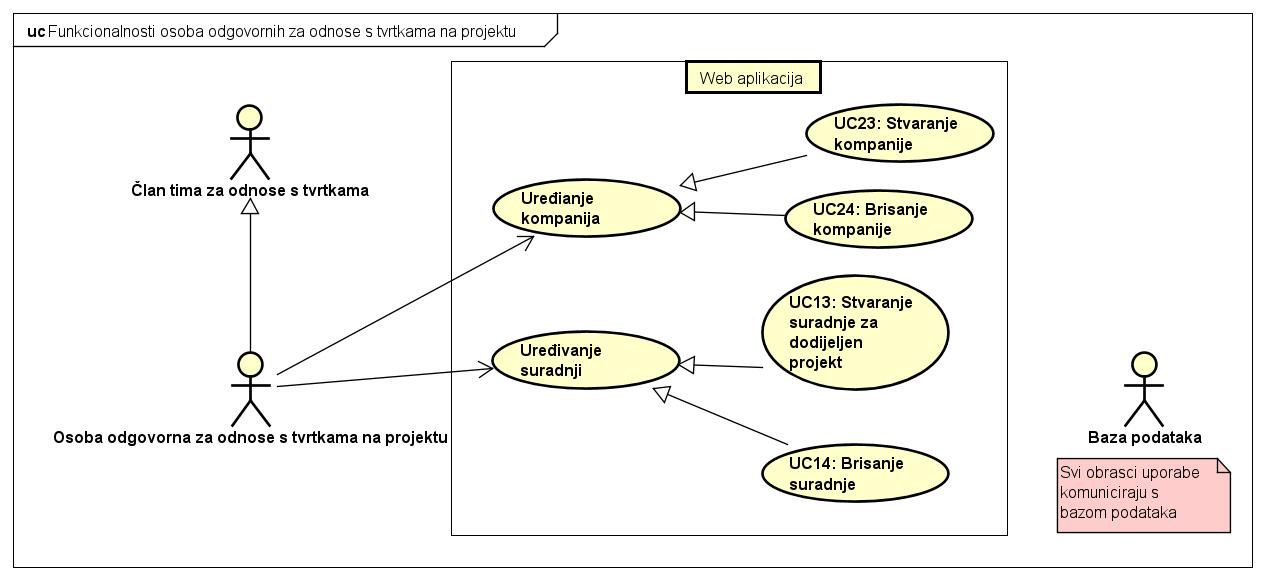
\includegraphics[scale=0.4]{slike/UC dijagrami/UseCase FR responsible}
						\centering
						\caption{Slika 3.3: Dijagram obrasca uporabe, funkcionalnosti osobe odgovorne za odnose s tvrtkama na projektu}
						\label{fig:frResponsible}
					\end{figure}

					\begin{figure}[H]
						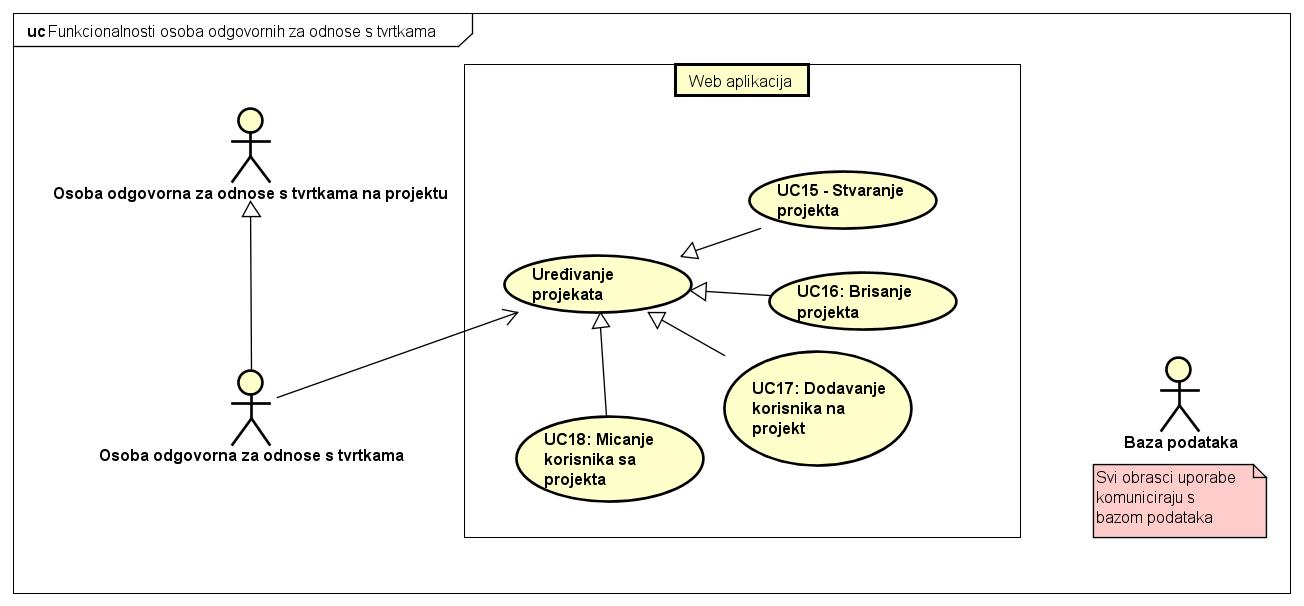
\includegraphics[scale=0.4]{slike/UC dijagrami/UseCase moderator}
						\centering
						\caption{Slika 3.4: Dijagram obrasca uporabe, funkcionalnosti osobe odgovorne za odnose s tvrtkama}
						\label{fig:frModerator}
					\end{figure}

					\begin{figure}[H]
						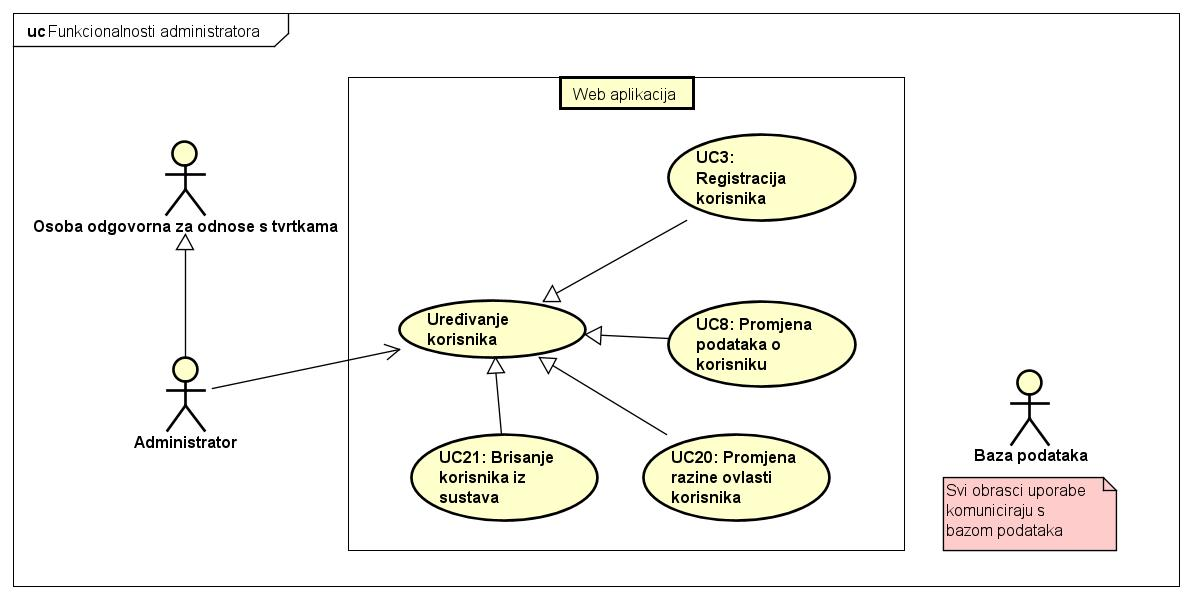
\includegraphics[scale=0.4]{slike/UC dijagrami/UseCase administrator}
						\centering
						\caption{Slika 3.5: Dijagram obrasca uporabe, funkcionalnosti administratora}
						\label{fig:administrator}
					\end{figure}

				\eject
				
			\subsection{Sekvencijski dijagrami}
				
				\textbf{\textit{dio 1. revizije}}\\
				
				\textit{Nacrtati sekvencijske dijagrame koji modeliraju najvažnije dijelove sustava (max. 4 dijagrama). Ukoliko postoji nedoumica oko odabira, razjasniti s asistentom. Uz svaki dijagram napisati detaljni opis dijagrama.}
				\eject
	
		\section{Ostali zahtjevi}
		
			\textbf{\textit{dio 1. revizije}}\\

			 \textit{Nefunkcionalni zahtjevi i zahtjevi domene primjene dopunjuju funkcionalne zahtjeve. Oni opisuju \textbf{kako se sustav treba ponašati} i koja \textbf{ograničenja} treba poštivati (performanse, korisničko iskustvo, pouzdanost, standardi kvalitete, sigurnost...). Primjeri takvih zahtjeva u Vašem projektu mogu biti: podržani jezici korisničkog sučelja, vrijeme odziva, najveći mogući podržani broj korisnika, podržane web/mobilne platforme, razina zaštite (protokoli komunikacije, kriptiranje...)... Svaki takav zahtjev potrebno je navesti u jednoj ili dvije rečenice.}\\

			\begin{packed_item}

				\item \textit{Sustav treba omogućiti rad više korisnika u stvarnom vremenu}
				\item \textit{Korisničko sučelje i sustav moraju podržavati hrvatsku abecedu (dijakritičke
				znakove) pri unosu i prikazu tekstualnog sadržaja}
				\item \textit{Izvršavanje dijela programa u kojem se pristupa bazi podataka ne smije trajati
				duže od nekoliko sekundi}
				\item \textit{Sustav treba biti implementiran kao web aplikacija koristeći
				objektno- orijentirane jezike}
				\item \textit{Neispravno korištenje korisničkog sučelja ne smije narušiti funkcionalnost i
				rad sustava}
				\item \textit{Sustav treba biti jednostavan za korištenje, korisnici se moraju znati koristiti
				sučeljem bez opširnih uputa}
				\item \textit{Veza s bazom podataka mora biti kvalitetno zaštičena, brza i otporna na
				vanjske greske}
				\item \textit{Pristup sustavu mora biti omogućen iz javne mreže pomoču HTTPS}
				\item \textit{Prikazivanje stranice korisniku ne smije trajati dulje od desetak sekundi,
				bez obzira na količinu podataka koju prikazuje}

			\end{packed_item}
			 
	
	Arhitektura i dizajn sustava}
		
		\textbf{\textit{dio 1. revizije}}\\

		\textit{ Potrebno je opisati stil arhitekture te identificirati: podsustave, preslikavanje na radnu platformu, spremišta podataka, mrežne protokole, globalni upravljački tok i sklopovsko-programske zahtjeve. Po točkama razraditi i popratiti odgovarajućim skicama:}
	\begin{itemize}
		\item 	\textit{izbor arhitekture temeljem principa oblikovanja pokazanih na predavanjima (objasniti zašto ste baš odabrali takvu arhitekturu)}
		\item 	\textit{organizaciju sustava s najviše razine apstrakcije (npr. klijent-poslužitelj, baza podataka, datotečni sustav, grafičko sučelje)}
		\item 	\textit{organizaciju aplikacije (npr. slojevi frontend i backend, MVC arhitektura) }		
	\end{itemize}

	
		

		

				
		\section{Baza podataka}
			
			\textbf{\textit{dio 1. revizije}}\\
			
		\textit{Podaci u našoj aplikaciji će se spremati u relacijsku bazu podataka koristeći Postgres kao DBMS. Baza će se sastojati od sljedećih entiteta:}
		\begin{itemize}
			\item Korisnik
			\item Tvrtka
			\item Projekt
			\item ProjectFRTeamMembers
			\item Mjesto
			\item Zaposlenik
			\item Suradnja
		\end{itemize}
			\subsection{Opis tablica}

				\begin{longtblr}[
					label=none,
					entry=none
					]{
						width = \textwidth,
						colspec={|X[14,l]|X[8, l]|X[20, l]|}, 
						rowhead = 1,
					} %definicija širine tablice, širine stupaca, poravnanje i broja redaka naslova tablice
						\hline \multicolumn{3}{|c|}{\textbf{Korisnik}}	 \\ \hline[3pt]
						\SetCell{LightGreen}IDKorisnik & INT & ID kosisnika  	\\ \hline
						Ime	& VARCHAR & Ime korisnika \\ \hline 
						Prezime & VARCHAR & Prezime korisnika \\ \hline 
						Nadimak & VARCHAR	& Nadimak korisnika \\ \hline 
        				LoginEmail & VARCHAR	& Email adresa pomoću kojeg se user logira \\ \hline 
        				NotificationEmail & VARCHAR	& Email adresa na koju korisnik prima obavijesti \\ \hline 
						MaxRazinaOvlasti & VARCHAR & Maksimalna razina ovlasti na projektima \\ \hline
				\end{longtblr}

				\begin{longtblr}[
					label=none,
					entry=none
					]{
						width = \textwidth,
						colspec={|X[14,l]|X[8, l]|X[20, l]|}, 
						rowhead = 1,
					} %definicija širine tablice, širine stupaca, poravnanje i broja redaka naslova tablice
						\hline \multicolumn{3}{|c|}{\textbf{Tvrtka}}	 \\ \hline[3pt]
						\SetCell{LightGreen} IdTvrtka & INT	&  Id tvrtke	\\ \hline
						Naziv & VARCHAR & Naziv tvrtke \\ \hline 
						Podrucje & VARCHAR &  Područje kojim se tvrtka bavi \\ \hline 
						ABCKategorija & CHAR & Kategorija tvrtke (A B ili C) \\ \hline 
		                MjesecPlaniranjaBudzeta & INT & Mjesec u kojem tvrtka planira budžet \\ \hline
		                Drzava & VARCHAR & Država u kojoj tvrtka posluje \\ \hline
		                \SetCell{LightBlue} PBr & VARCHAR & Poštanski broj mjesta tvrtke \\ \hline
						Adresa & VARCHAR & Adresa tvrtke \\ \hline
	                 	WebStranica & VARCHAR & Adresa web stranice tvrtke \\ \hline
		                Kontaktirati & BOOLEAN & Treba li ubuduće tu tvrtku treba kontaktirati \\ \hline
				\end{longtblr}

				\begin{longtblr}[
					label=none,
					entry=none
					]{
						width = \textwidth,
						colspec={|X[14,l]|X[8, l]|X[20, l]|}, 
						rowhead = 1,
					} %definicija širine tablice, širine stupaca, poravnanje i broja redaka naslova tablice
					\hline \multicolumn{3}{|c|}{\textbf{Projekt}}	 \\ \hline[3pt]
					\SetCell{LightGreen}IDProjekt & INT	& Id projekta \\ \hline
					Naziv & VARCHAR & Naziv projekta \\ \hline 
					KategorijaProjekta & INT & Kategorija u koju spada projekt \\ \hline 
					TipProjekta & VARCHAR & Eksterni ili interni projekt \\ \hline 
					DatumPočetka & TIMESTAMP & Datum početka projekta \\ \hline 
	                DatumZavršetka & TIMESTAMP & Datum završetka projekta \\ \hline 
	                \SetCell{LightBlue} FRResponsibleUserId & INT & Id korisnika odgovornog za odnose s tvrtkama projekta \\ \hline
	                FRCilj & INT & Količina novca koja se želi prikupiti za projekt \\ \hline
	                FirstPing & TIMESTAMP & Datum prvog "ping"-a \\ \hline
	                SecondPing & TIMESTAMP & Datum drugog "ping"-a \\ \hline
				\end{longtblr}

				\begin{longtblr}[
					label=none,
					entry=none
					]{
						width = \textwidth,
						colspec={|X[14,l]|X[8, l]|X[20, l]|}, 
						rowhead = 1,
					} %definicija širine tablice, širine stupaca, poravnanje i broja redaka naslova tablice
					\hline \multicolumn{3}{|c|}{\textbf{TipProjekta}}	 \\ \hline[3pt]
					\SetCell{LightGreen}IDTipProjekt & INT	& Id tipa projekta \\ \hline
					TipProjekta	& VARCHAR & Tip projekta \\ \hline 
				\end{longtblr}

				\begin{longtblr}[
					label=none,
					entry=none
					]{
						width = \textwidth,
						colspec={|X[14,l]|X[8, l]|X[20, l]|}, 
						rowhead = 1,
					} %definicija širine tablice, širine stupaca, poravnanje i broja redaka naslova tablice
					\hline \multicolumn{3}{|c|}{\textbf{ProjectFRTeamMembers}}	 \\ \hline[3pt]
					\SetCell{LightGreen}IDKorisnik & INT & Id korisnika koji je FR team member projekta \\ \hline
					\SetCell{LightGreen}IDProjekt & INT & Id projekta \\ \hline
				\end{longtblr}

				\begin{longtblr}[
					label=none,
					entry=none
					]{
						width = \textwidth,
						colspec={|X[14,l]|X[8, l]|X[20, l]|}, 
						rowhead = 1,
					} %definicija širine tablice, širine stupaca, poravnanje i broja redaka naslova tablice
					\hline \multicolumn{3}{|c|}{\textbf{Mjesto}}	 \\ \hline[3pt]
					\SetCell{LightGreen} PostanskiBrojGrad & VARCHAR & Poštanski broj grada \\ \hline
					NazivGrad & VARCHAR & Naziv grada \\ \hline
				\end{longtblr}

				\begin{longtblr}[
					label=none,
					entry=none
					]{
						width = \textwidth,
						colspec={|X[14,l]|X[8, l]|X[20, l]|}, 
						rowhead = 1,
					} %definicija širine tablice, širine stupaca, poravnanje i broja redaka naslova tablice
					\hline \multicolumn{3}{|c|}{\textbf{Zaposlenik}}	 \\ \hline[3pt]
						\SetCell{LightGreen} IDZaposlenik & INT	& Id zaposlenika \\ \hline
						\SetCell{LightBlue} IDTvrtke & INT & Id tvrtke za koju zaposlenik radi\\ \hline 
						Ime & VARCHAR & Ime zaposlenika \\ \hline 
						Prezime & VARCHAR	& Prezime zaposlenika \\ \hline 
	                    Email & VARCHAR	& Email adresa zaposlenika \\ \hline 
	                    BrojTelefona & VARCHAR	& Broj telefona zaposlenika \\ \hline 
	                    Uloga & VARCHAR	& Pozicija zaposlenika u tvrtci (npr. PR) \\ \hline 
	                    Opis & VARCHAR	& Opis zaposlenika (npr. glavni kontakt) \\ \hline 
				\end{longtblr}

				\begin{longtblr}[
					label=none,
					entry=none
					]{
						width = \textwidth,
						colspec={|X[14,l]|X[8, l]|X[20, l]|}, 
						rowhead = 1,
					} %definicija širine tablice, širine stupaca, poravnanje i broja redaka naslova tablice
					\hline \multicolumn{3}{|c|}{\textbf{Suradnja}}	 \\ \hline[3pt]
					\SetCell{LightGreen}IDProjekt & INT	& Id projekta \\ \hline
			                \SetCell{LightGreen}IdTvrtke & INT	& Id tvrtke \\ \hline
					\SetCell{LightBlue}IdOdgovoran & INT & Id korisnika odgovornog za suradnju s tvrtkom \\ \hline 
					\SetCell{LightBlue}IdKontakt & INT & Id kontakt osobe u tvrtci \\ \hline 
					KategorijaSuradnje & VARCHAR & Kategorija suradnje (Financijska, materijalna ili akademska) \\ \hline
		                    Status & VARCHAR & Kontaktirano, ping, dopis, sastanak, uspješno ili neuspješno \\ \hline
		                    Komentar & VARCHAR & Komentar na suradnju \\ \hline
		                    VrijednostSuradnje & FLOAT & Novčana vrijednost suradnje \\ \hline
				\end{longtblr}
				
			
			\subsection{Dijagram baze podataka}
				\begin{figure}[H]
					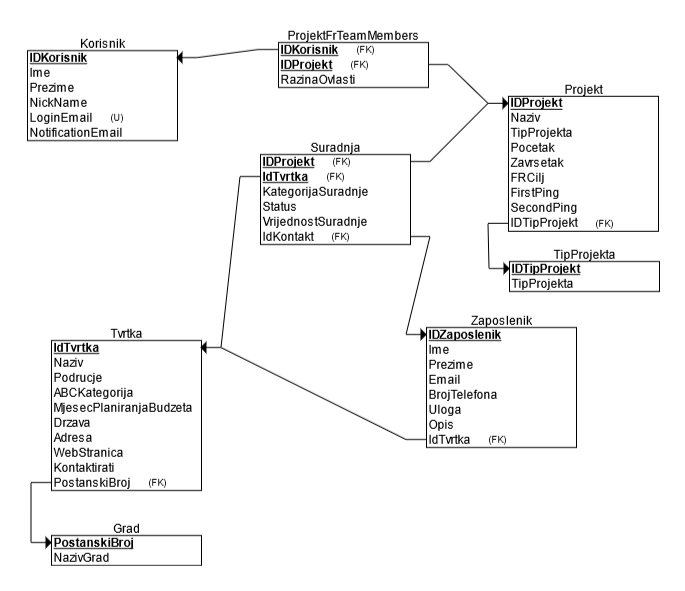
\includegraphics[scale=0.6]{DBDiagram}
					\centering
					\caption{Database Diagram}
					\label{fig:dbdiagram}
				\end{figure}
			\eject
			
			
		\section{Dijagram razreda}
		
			Na sljedećim slikama prikazani su UML dijagrami razreda koji se koriste u aplikaciji. Podijeljeni su u 3 dijela. Prvi dijagram prikazuje klase kojima smo modelirali entitete aplikacije, drugi prikazuje DTO-ove\textit{(Data transfer object)}, a treći prikazuje Controllere. Može se uočiti da postoje veze između klasa iz različitih dijagrama(npr. UserDto sadrži UserSystemAuthority), ali su one izostavljene radi preglednosti.
			\begin{figure}[H]
				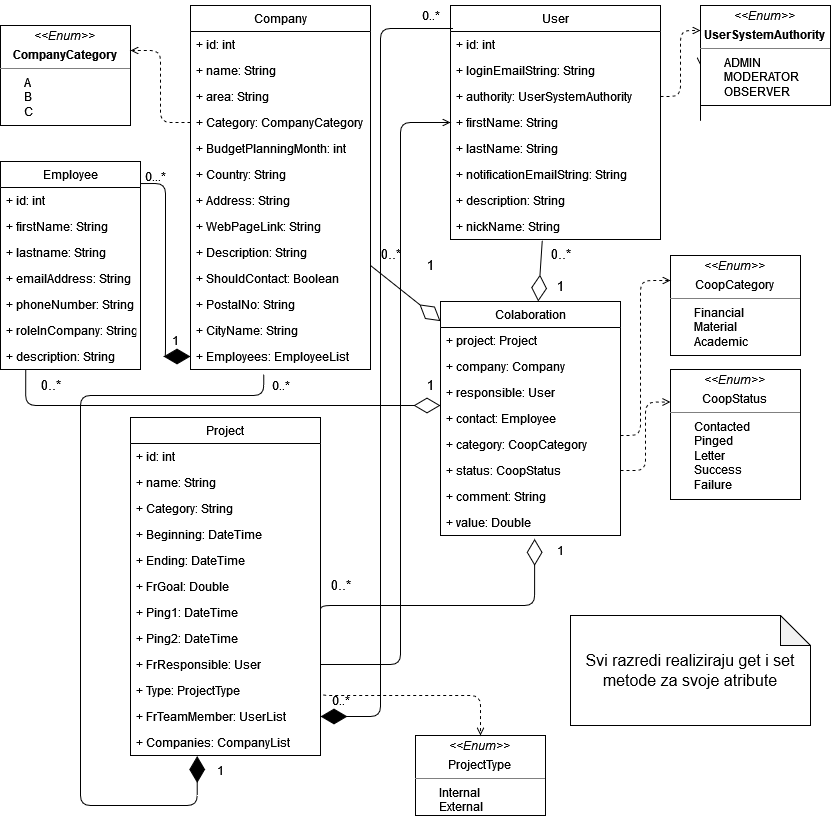
\includegraphics[scale=0.5]{ModelUml} %veličina slike u odnosu na originalnu datoteku i pozicija slike
				\centering
				\caption{Models UML}
				\label{fig:modelUml}
			\end{figure}
			\begin{figure}[H]
				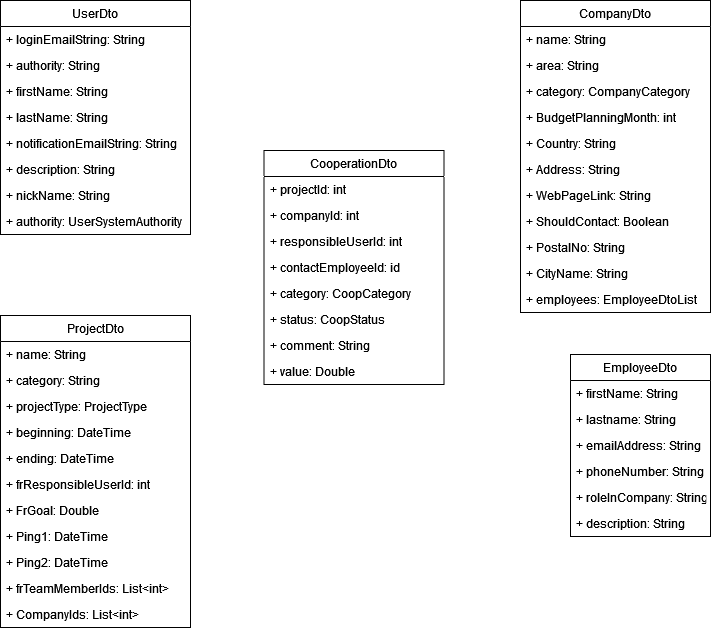
\includegraphics[scale=0.5]{DtoUml} %veličina slike u odnosu na originalnu datoteku i pozicija slike
				\centering
				\caption{DtoUml}
				\label{fig:dtouml}
			\end{figure}
			\begin{figure}[H]
				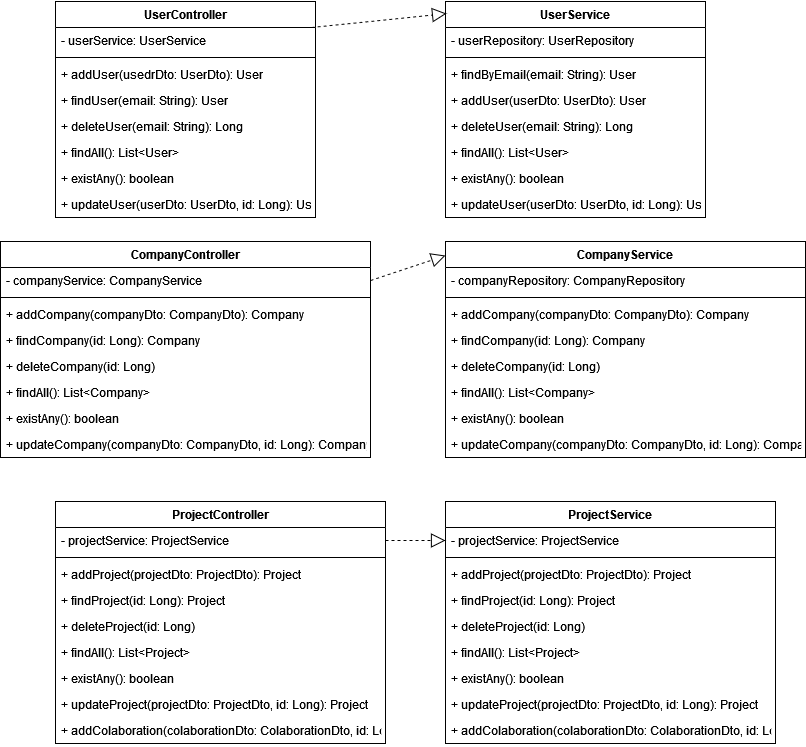
\includegraphics[scale=0.5]{ControllerServiceUml} %veličina slike u odnosu na originalnu datoteku i pozicija slike
				\centering
				\caption{Controllers and services UML}
				\label{fig:controllersServicesUml}
		\end{figure}
		\section{Dijagram stanja}
			
			
			\textbf{\textit{dio 2. revizije}}\\
			
			\textit{Potrebno je priložiti dijagram stanja i opisati ga. Dovoljan je jedan dijagram stanja koji prikazuje \textbf{značajan dio funkcionalnosti} sustava. Na primjer, stanja korisničkog sučelja i tijek korištenja neke ključne funkcionalnosti jesu značajan dio sustava, a registracija i prijava nisu. }
			
			
			\eject 
		
		\section{Dijagram aktivnosti}
			
			\textbf{\textit{dio 2. revizije}}\\
			
			 \textit{Potrebno je priložiti dijagram aktivnosti s pripadajućim opisom. Dijagram aktivnosti treba prikazivati značajan dio sustava.}
			
			\eject
		\section{Dijagram komponenti}
		
			\textbf{\textit{dio 2. revizije}}\\
		
			 \textit{Potrebno je priložiti dijagram komponenti s pripadajućim opisom. Dijagram komponenti treba prikazivati strukturu cijele aplikacije.}
	\chapter{Implementacija i korisničko sučelje}
		
		\section{Korištene tehnologije i alati}
		
			% \textbf{\textit{dio 2. revizije}}
			
			%  \textit{Detaljno navesti sve tehnologije i alate koji su primijenjeni pri izradi dokumentacije i aplikacije. Ukratko ih opisati, te navesti njihovo značenje i mjesto primjene. Za svaki navedeni alat i tehnologiju je potrebno \textbf{navesti internet poveznicu} gdje se mogu preuzeti ili više saznati o njima}.

            {Većinski dio komunikacije održan je putem WhatsApp\footnotemark{}\footnotetext{https://www.whatsapp.com/} komunikacijskog kanala, dok je drugi dio održan ili uživo ili preko platforme Discord\footnotemark{}\footnotetext{https://discord.com/}. Prilikom izrade dijagrama korišten je alat Astah\footnotemark{}\footnotetext{https://astah.net/}, dok je za pisanje dokumentacije korišten online editor Overleaf\footnotemark{}\footnotetext{https://www.overleaf.com/}.}\vspace{0.3cm}

            {U svrhu verzioniranja koda od strane svih članova grupe korišten je alat Git\footnotemark{}\footnotetext{https://git-scm.com/}, dok je kao udaljeni repozitorij korištena platforma GitLab\footnotemark{}\footnotetext{https://gitlab.com/}.}\vspace{0.2cm}
            
            {Za razvoj Backend dijela aplikacije korišten je Java JDK\footnotemark{}\footnotetext{https://www.oracle.com/java/technologies/downloads/}, gradle\footnotemark{}\footnotetext{https://gradle.org/} i Intellij Idea\footnotemark{}\footnotetext{https://www.jetbrains.com/idea/} razvojno okruženje za razvoj Spring boot\footnotemark{}\footnotetext{https://spring.io/projects/spring-boot} aplikacije. Za Frontend dio aplikacije korišten je Node.js\footnotemark{}\footnotetext{https://nodejs.org/en/} kao program za pokretanje i React\footnotemark{}\footnotetext{https://reactjs.org/}, također poznat kao React.js ili ReactJS, kao Javascript\footnotemark{}\footnotetext{https://www.javascript.com/} bibiloteka za izradu sučelja. Kao razvojno okruženje za React korišten je VS Code\footnotemark{}\footnotetext{https://code.visualstudio.com/} IDE.}\vspace{0.3cm}
            
            {Za upravljanje bazom podataka korišten je PostgreSQL\footnotemark{}\footnotetext{https://www.postgresql.org/} instaliran na Ubuntu serveru\footnotemark{}\footnotetext{https://ubuntu.com/download/server} verzije 20.04.}
			
			\eject 
		
	
		\section{Ispitivanje programskog rješenja}
			
			\subsection{Ispitivanje komponenti}
			{Svi endpointovi na backend-u su ručno testirani, a ispitivanje jedinica (engl. unit testing) proveli smo nad osnovnim funkcionalnostima servisnog sloja koristeći biblioteku junit. Prilikom testiranja pojedinog razreda, servise i repozitorije čije metode taj razred poziva smo \textit{mock-ali} koristeći biblioteku mockito, pa smo samo u svakoj test metodi zadali što će pojedina pozvana metoda vraćati.}
			
			\textbf{1. UserServiceTests\\}
			{U UserServiceTests testnoj klasi ispitali smo funkcionalnost dodavanja novog korisnika u bazu podataka.\\
			Naredbom \textit{Mockito.when(userRepository.save(Mockito.any())).thenReturn(test);} smo rekli mockanom userRepository-ju kako da se ponaša prilikom poziva save metode.}
			\begin{figure}[H]
				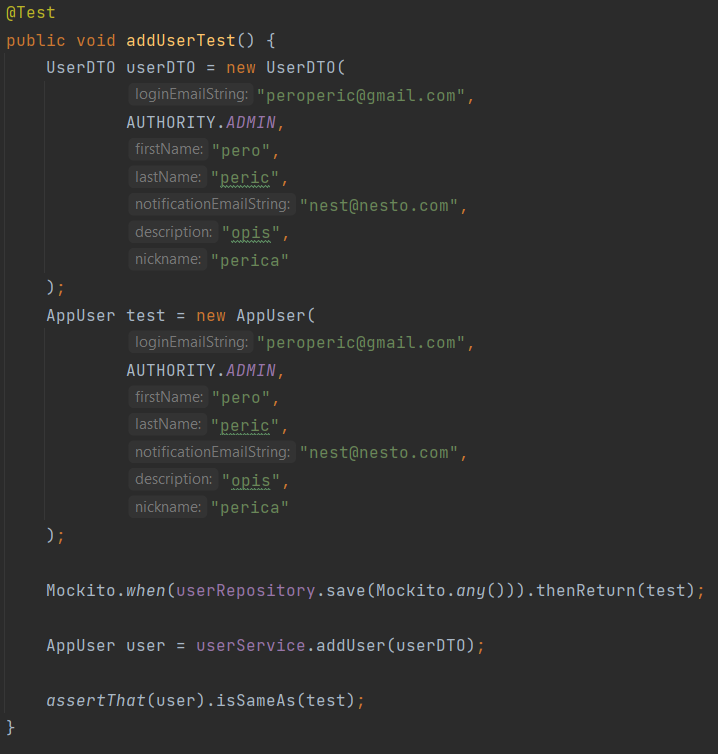
\includegraphics[width=\textwidth]{UnitTests/addUserTest}
				\centering
				\caption{Add user test}
				\label{fig:addUserTest}
			\end{figure}
			\begin{figure}[H]
				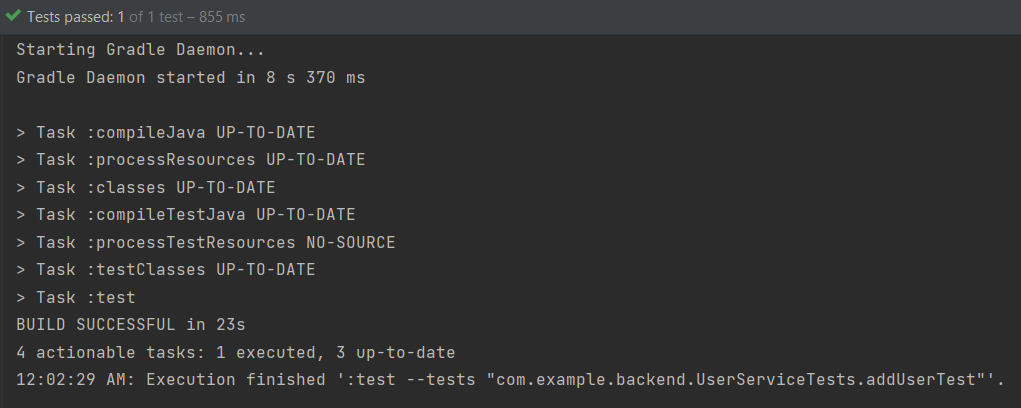
\includegraphics[width=\textwidth]{UnitTests/addUserTestResult}
				\centering
				\caption{Add user test result}
				\label{fig:addUserTestResult}
			\end{figure}
			
			\textbf{2. ProjectServiceTests\\}
			{U ProjectServiceTests klasi smo ispitali funkcionalnosti dohvata projekta iz baze podataka te dodavanje FR team membera na projekt.}
			\begin{figure}[H]
				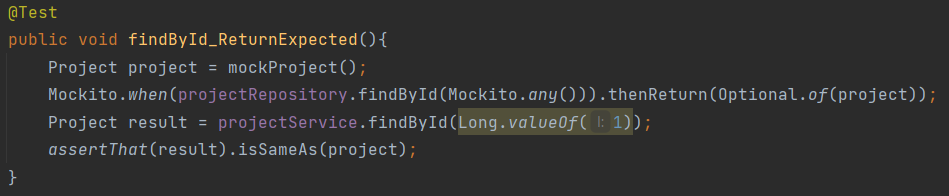
\includegraphics[width=\textwidth]{UnitTests/projectFindById}
				\centering
				\caption{Find project by Id test}
				\label{fig:projectFindByIdTest}
			\end{figure}
			\begin{figure}[H]
				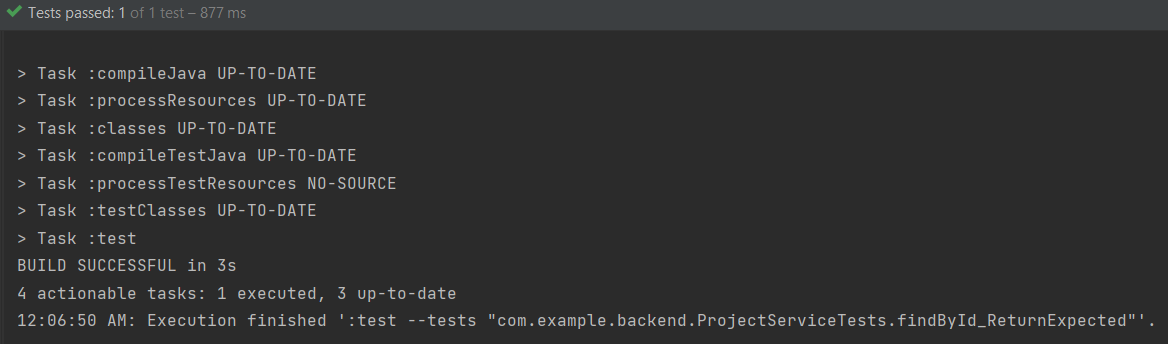
\includegraphics[width=\textwidth]{UnitTests/projectFindByIdResult}
				\centering
				\caption{Find project by Id test result}
				\label{fig:projectFindByIdResult}
			\end{figure}

			\begin{figure}[H]
				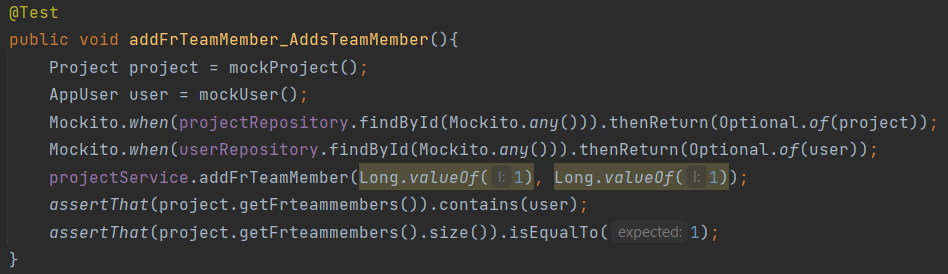
\includegraphics[width=\textwidth]{UnitTests/projectAddFrTeamMember}
				\centering
				\caption{Add FR team member to project test}
				\label{fig:addFrTeamMemberTest}
			\end{figure}
			\begin{figure}[H]
				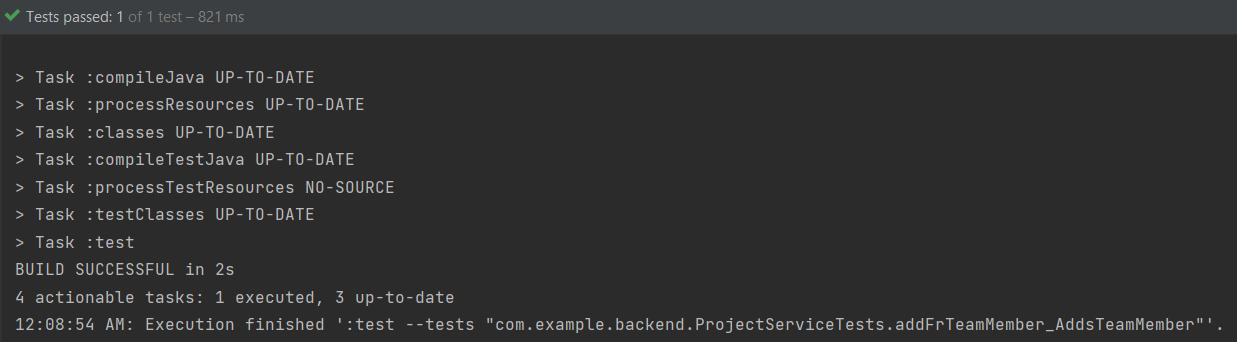
\includegraphics[width=\textwidth]{UnitTests/projectAddFrTeamMemberResult}
				\centering
				\caption{Add FR team member result}
				\label{fig:addFrTeamMemberResult}
			\end{figure}

			\textbf{3. CompanyServiceTests\\}
			{U CompanyServiceTests klasi smo ispitali sljedeće funkcionalnosti:\\
				Kreiranje nove kompanije\\
				Dohvaćanje svih kompanije\\
				Bacanje EntityNotFoundException-a prilikom pokušaja brisanja nepostojeće kompanije\\
				Bacanje AuthenticationException-a prilikom pokušaja dohvata podataka od kompanije od strane Usera koji je samo Observer}
			
			\begin{figure}[H]
				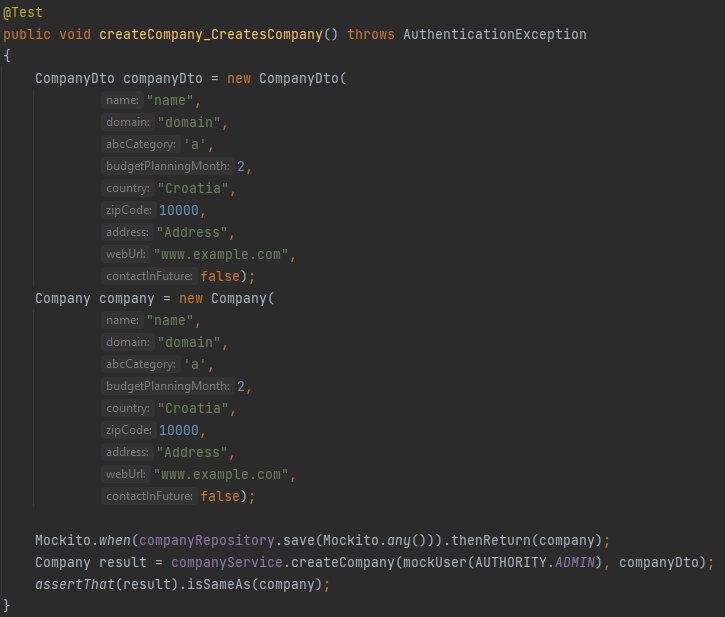
\includegraphics[width=\textwidth]{UnitTests/createCompany}
				\centering
				\caption{Create company test}
				\label{fig:createCompanyTest}
			\end{figure}
			\begin{figure}[H]
				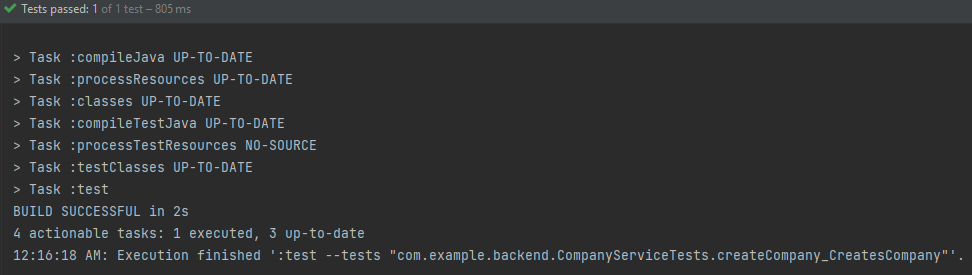
\includegraphics[width=\textwidth]{UnitTests/createCompanyResult}
				\centering
				\caption{Create company test result}
				\label{fig:createCompanyResult}
			\end{figure}

			\begin{figure}[H]
				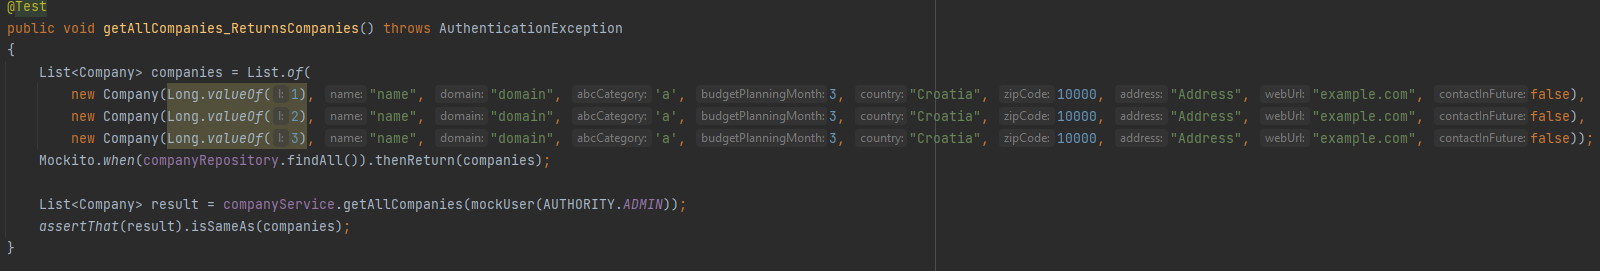
\includegraphics[width=\textwidth]{UnitTests/getAllCompanies}
				\centering
				\caption{Get all companies test}
				\label{fig:getAllCompaniesTest}
			\end{figure}
			\begin{figure}[H]
				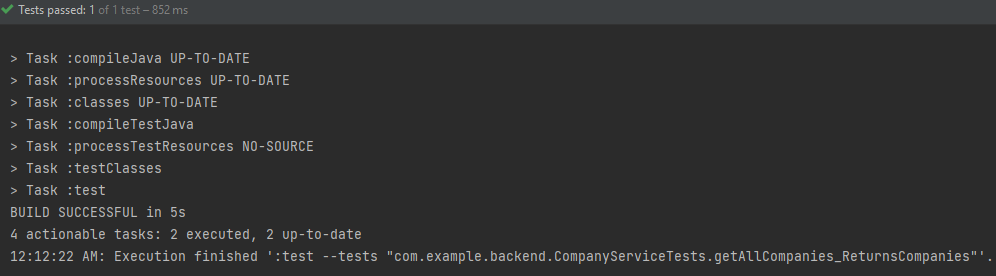
\includegraphics[width=\textwidth]{UnitTests/getAllCompaniesResult}
				\centering
				\caption{Get all companies test result}
				\label{fig:getAllCompaniesResult}
			\end{figure}

			\begin{figure}[H]
				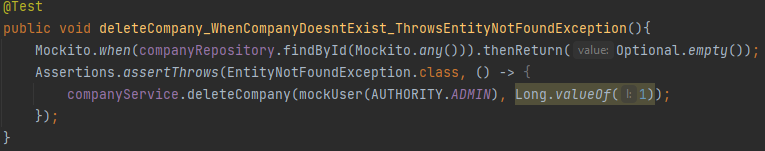
\includegraphics[width=\textwidth]{UnitTests/deleteCompanDoesntExist}
				\centering
				\caption{Delete company which does not exist test}
				\label{fig:deleteCompanyTest}
			\end{figure}
			\begin{figure}[H]
				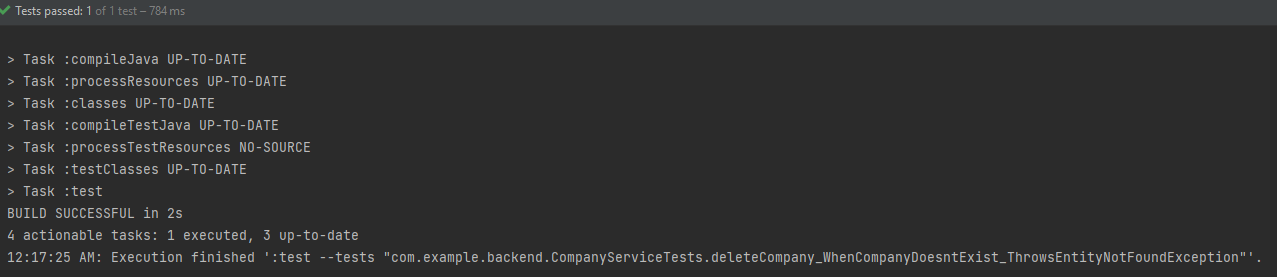
\includegraphics[width=\textwidth]{UnitTests/deleteCompanDoesntExistResult}
				\centering
				\caption{Delete company which does not exist tes result}
				\label{fig:deleteCompanyResult}
			\end{figure}

			\begin{figure}[H]
				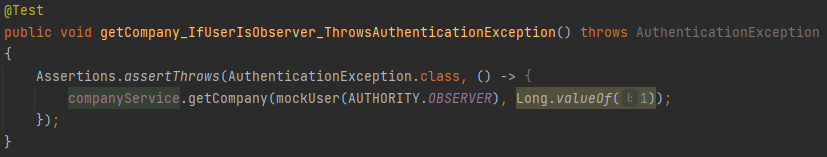
\includegraphics[width=\textwidth]{UnitTests/getCompanyObserver}
				\centering
				\caption{Get company info by observer test}
				\label{fig:getCompanyObserver}
			\end{figure}
			\begin{figure}[H]
				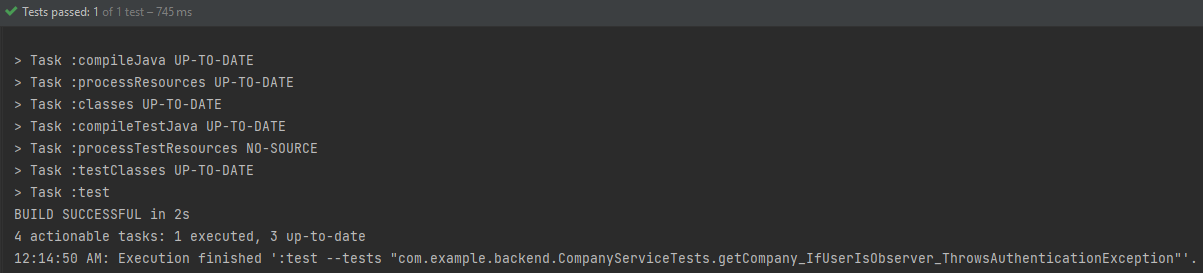
\includegraphics[width=\textwidth]{UnitTests/getCompanyObserverResult}
				\centering
				\caption{Get company info by observer test result}
				\label{fig:getCompanyObserverResult}
			\end{figure}
			
			\textbf{4. CollaborationServiceTests\\}
			{U CollaborationServiceTests testnoj klasi smo ispitali funkcionalnost dodavanja suradnje u bazu podataka.}

			\begin{figure}[H]
				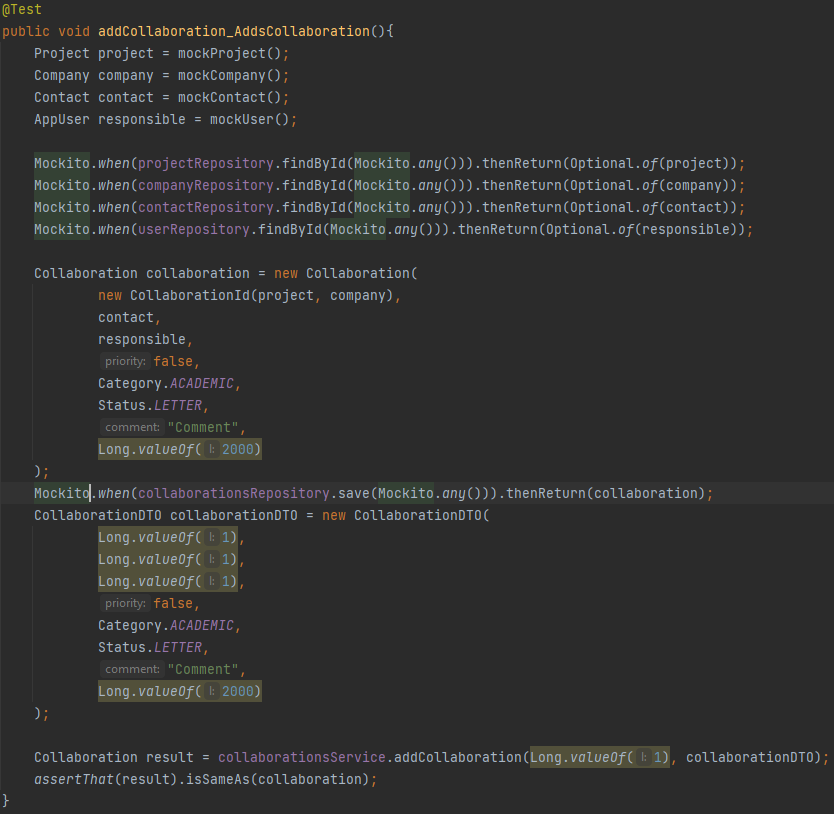
\includegraphics[width=\textwidth]{UnitTests/addCollaboration}
				\centering
				\caption{Add collaboration test}
				\label{fig:addCollaboration}
			\end{figure}
			\begin{figure}[H]
				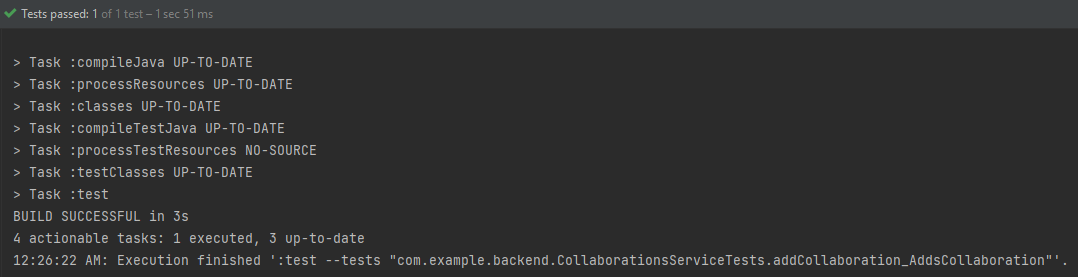
\includegraphics[width=\textwidth]{UnitTests/addCollaborationResult}
				\centering
				\caption{Add collaboration test result}
				\label{fig:addCollaborationResult}
			\end{figure}

			% \subsection{Ispitivanje sustava}
			
			%  \textit{Potrebno je provesti i opisati ispitivanje sustava koristeći radni okvir Selenium\footnote{\url{https://www.seleniumhq.org/}}. Razraditi \textbf{minimalno 4 ispitna slučaja} u kojima će se ispitati redovni slučajevi, rubni uvjeti te poziv funkcionalnosti koja nije implementirana/izaziva pogrešku kako bi se vidjelo na koji način sustav reagira kada nešto nije u potpunosti ostvareno. Ispitni slučaj se treba sastojati od ulaza (npr. korisničko ime i lozinka), očekivanog izlaza ili rezultata, koraka ispitivanja i dobivenog izlaza ili rezultata.\\ }
			 
			%  \textit{Izradu ispitnih slučajeva pomoću radnog okvira Selenium moguće je provesti pomoću jednog od sljedeća dva alata:}
			%  \begin{itemize}
			%  	\item \textit{dodatak za preglednik \textbf{Selenium IDE} - snimanje korisnikovih akcija radi automatskog ponavljanja ispita	}
			%  	\item \textit{\textbf{Selenium WebDriver} - podrška za pisanje ispita u jezicima Java, C\#, PHP koristeći posebno programsko sučelje.}
			%  \end{itemize}
		 % 	\textit{Detalji o korištenju alata Selenium bit će prikazani na posebnom predavanju tijekom semestra.}
			
			\eject 
		
		
		\section{Dijagram razmještaja}
			
			{ Na poslužiteljskom računalu se nalaze web poslužitelj i poslužitelj baze podataka. Klijenti koriste web
			preglednik kako bi pristupili web aplikaciji. Sustav je baziran na arhitekturi ”klijent – poslužitelj”, a
			komunikacija između računala korisnika (klijent, zaposlenik, vlasnik, administrator) i poslužitelja odvija se preko HTTP veze. }

			\begin{figure}[H]
				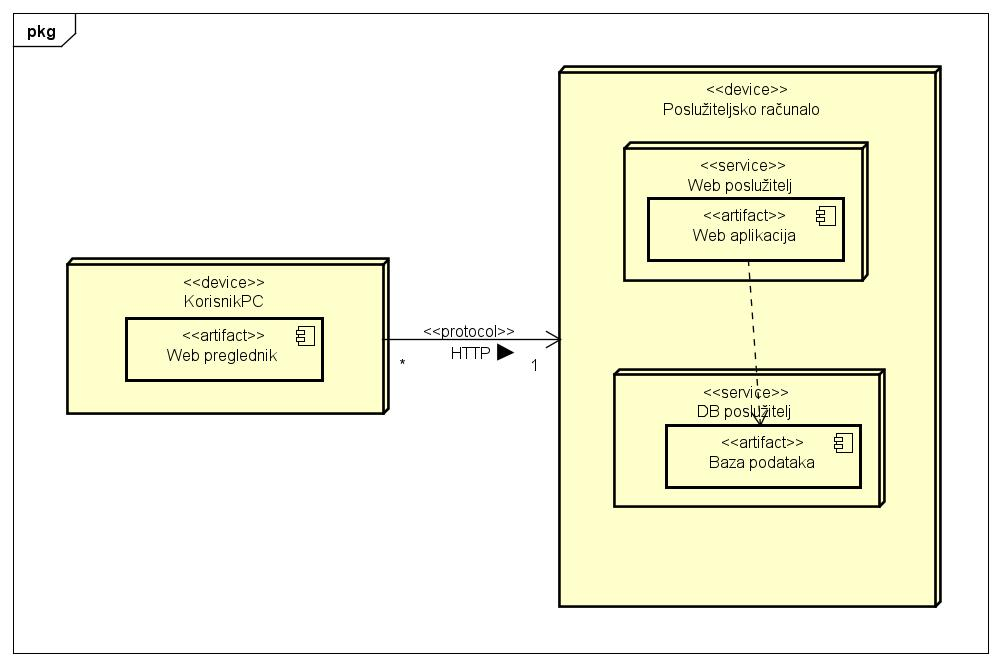
\includegraphics[width=\textwidth]{slike/Dijagram razmjestaja}
				\centering
				\caption{Dijagram razmještaja}
				\label{fig:razmijestaja}
			\end{figure}

			\eject 
		
		\section{Upute za puštanje u pogon}
		
            {Kako se aplikacija sastoji od dva distinktivna dijela, backend-a i frontend-a, svaki dio funkcionira samo za sebe te se zasebno pušta u pogon.}

			\subsection{Backend}

                {Backend se sastoji od koda u obliku gradle projekta u rađenom u Spring boot okruženju. Kako Spring boot samostalno radi tablice i ažurira relacije u bazi podataka, potrebno je samo na poslužitelju na kojem će se nalaziti kompajliran pokrenut kod stvoriti bazu podataka s nazivom \textit{cdb}.}
                
                {Za početak je potrebno otvoriti virtualni stroj s ubuntu serverom na poslužitelju po izboru nakon čega je potrebno unesti sljedeće naredbe koristeći command prompt kako bi se ulogirali i postavili server:}

                \begin{packed_item}
        			\item {ssh root@ipv4AdresaServera}
        			\item {sudo apt update}
        			\item {sudo apt upgrade}
        			\item {sudo apt install fail2ban}
        			\item {sudo systemctl restart fail2ban.service}
        		\end{packed_item}

                {Sada kada je server postavljen, potrebno je instalirati postgresql i podignuti bazu naziva cdb:}

                \begin{packed_item}
        			\item {sudo apt-get install postgresql postgresql-contrib}
        			\item {sudo systemctl start postgresql.service}
        			\item {sudo systemctl enable postgresql.service}
        			\item {sudo -u postgres psql}
        			\item {\textbackslash password postgres}
        			\item {CREATE DATABASE cdb}
        			\item {\textbackslash c cdb}
        			\item {\textbackslash q}
        		\end{packed_item}

                {Nakon što je baza podataka na serveru stvorena, potrebno je kompajlirati kod za backend aplikacije te ga tako kompajliranog prebaciti na server. Sljedeće naredbe potrebno je izvršiti u matičnog folderu koda preuzetnog na vlastito računalo:}

                \begin{packed_item}
        			\item {cd Backend}
        			\item {gradle bootJar}
        			\item {scp build/libs/backend-0.0.1-SNAPSHOT.jar root@ipv4AdresaServera:/var/www}
        		\end{packed_item}

                {Nakon što je kompajlirani kod na serveru, potrebno je instalirati javu kako bi ga mogli pokrenuti:}

                \begin{packed_item}
        			\item {sudo apt install openjdk-17-jdk}
        		\end{packed_item}

                {Kako bi osigurali da aplikacija radi i kada na serveru ne postoji ulogirani korisnik, potrebno je kompajliran kod pokrenuti kao servis:}

                \begin{packed_item}
        			\item {cd /usr/lib/systemd/system}
        			\item {nano runSpringServer.service}
        			\item \textit{Sljedeći kod upiši u novootvoreni text editor:}
        			\item {[Unit]}
                    \item {Description=webserver Daemon}
                    \item {[Service]}
                    \item {ExecStart=/usr/bin/java -jar /var/www/backend-0.0.1-SNAPSHOT.jar}
                    \item {User=root}
                    \item {[Install]}
                    \item {WantedBy=multi-user.target}
        			\item \textit{Zatvori text editor koristeći kombinacije tipki CTRL+S pa CTRL+X.}
        			\item {sudo systemctl start runSpringServer.service}
        			\item {sudo systemctl enable runSpringServer.service}
        		\end{packed_item}

            \subsection{Frontend}

                {Frontend je aplikacija rađena u React frameworku za čije je pokretanje i izgradnju potreban \textit{Node.js} koji je moguće preuzeti s adrese \textit{https://nodejs.org/en/download/}. Nakon instalacije \textit{Node.js}-a na vlastito računalo, u matičnom folderu koda preuzetog na vlastito računalo potrebno je izvršiti sljedeće naredbe kako bi kompajlirali frontend dio aplikacije:}

                \begin{packed_item}
        			\item {cd Frontend}
        			\item {npm install}
        			\item {npm run build}
        		\end{packed_item}

              {Nakon izvršenja ovih naredbi, u mapi Frontend će se stvoriti nova mapa naziva \textit{Build}. Ovu mapa sadrži kompajlirani kod Frontend aplikacije koji će biti potrebno prenesti na poslužitelj.}\vspace{0.3cm}

              {Kako bi korisnici kroz preglednik mogli pristupiti našoj aplikaciji potrebno ju je servirati na poslužitelju. Poslužitelj s kojeg će biti servirana naša aplikacija zove se \textit{Netlify}. Prvo je potrebno otići na adresu \textit{https://app.netlify.com/} i ulogirati se s već postojećim Github računom. Nakon toga potrebno je odabrati opciju \textit{Add new site} pa \textit{Deploy manually}. Prateći ove upute biti će ponuđen ekran na koji je potrebno ispustiti \textit{Build} mapu napravljenu u prethodnom koraku.}

              {Nakon nekoliko minuta Frontend aplikacija će se poslužiti te će nam Netlify dati IP adresu preko koje možemo pristupiti svojoj aplikaciji \textit{(npr. https://darling-lokum-558ee5.netlify.app)}.}\vspace{0.3cm}
              
              {Po želji, preteći Netlify dokumentaciju moguće je promijeniti IP adresu aplikacije kao i mnoge druge postavke koje Netlify nudi, no koji nisu potrebne za funkcioniranje aplikacije.}
			\eject 
	\chapter{Zaključak i budući rad}
	
	% \textbf{\textit{dio 2. revizije}}\\
	
	% 	\textit{U ovom poglavlju potrebno je napisati osvrt na vrijeme izrade projektnog zadatka, koji su tehnički izazovi prepoznati, jesu li riješeni ili kako bi mogli biti riješeni, koja su znanja stečena pri izradi projekta, koja bi znanja bila posebno potrebna za brže i kvalitetnije ostvarenje projekta i koje bi bile perspektive za nastavak rada u projektnoj grupi.}
	
	% 	\textit{Potrebno je točno popisati funkcionalnosti koje nisu implementirane u ostvarenoj aplikaciji.}

	{Zadatak naše grupe bio je razvoj web aplikacije koja bi služila neprofitnim organizacijama kao baza podataka projekata i kompanija s kojima se surađivalo na istim. Nakon 12 tjedana rada u timu i razvoja, približno smo ostvarili zadani cilj. Sama provedba projekta bila je kroz dvije faze.}

	{Prva faza projekta uključivala je okupljanje tima za razvoj aplikacije, dodjelu projektnog zadatka i intenzivan rad na dokumentiranju zahtjeva. Kvalitetna provedba prve faze uvelike je olakšala daljnji rad pri realizaciji osmišljenog sustava. Izrađeni obrasci i dijagrami (obrasci uporabe, sekvencijski dijagrami, model baze podataka, dijagram razreda) bili su od pomoći podtimovima zaduženima za razvoj backenda i frontenda. Izrada vizualnih prikaza idejnih rješenja problemskog zadatka uštedjela je mnogo vremena u drugom ciklusu kada su članovi tima nailazili na nedoumice oko implementacije rješenja.}

	{Druga faza projekta, iako nešto kraća od prve, bila je puno intenzivnija po pitanju samostalnog rada članova. Manjak iskustva članova u izradi sličnih implementacijskih rješenja primorao je članove na samostalno učenje odabranih alata i programskih jezika kako bi ispunili dogovorene ciljeve. Osim realizacije rješenja, u drugoj fazi je bilo potrebno dokumentirati ostale UML dijagrame i izraditi popratnu dokumentaciju kako bi budući korisnici mogli lakše koristiti ili vršiti preinake na sustavu. Dobro izrađen kostur projekta uštedio nam je mnogo vremena prilikom izrade aplikacije te smo izbjegli moguće pogreške u izradi koje bi bile vremenski skupe za ispravljanje u daljnjoj fazi projekta. Komunikacija među članovima tima bila je putem WhatsAppa čime smo postigli informiranost svih članova grupe o napretku projekta. Moguće proširenje postojeće inačice sustava je izrada mobilne aplikacije čime bi se cilj projektnog zadatka bio ostvaren u većoj mjeri no s web aplikacijom. Sudjelovanje na ovakvom projektu bilo je vrijedno iskustvo svim članovima tima jer smo kroz intenzivnih nekoliko tjedana rada iskusili zajednički rad na istom projektu. Također, osjetili smo važnost dobre vremenske organiziranosti i koordiniranosti između članova tima.}
	
	{Zadovoljni smo postignutim bez obzira na golemi prostor za usavršavanje izrađene aplikacije što je posljedica neiskustva na takvim i sličnim projektima.}
	
	\eject
	\chapter*{Popis literature}
		\addcontentsline{toc}{chapter}{Popis literature}
	 	
    %    \textbf{\textit{Kontinuirano osvježavanje}}
	
	%	\textit{Popisati sve reference i literaturu koja je pomogla pri ostvarivanju projekta.}
		
		\begin{enumerate}
			\item  Programsko inženjerstvo, FER ZEMRIS, \url{http://www.fer.hr/predmet/proinz}
			
			\item  I. Sommerville, "Software engineering", 8th ed, Addison Wesley, 2007.
			
			\item  T.C.Lethbridge, R.Langaniere, "Object-Oriented Software Engineering", 2nd ed. McGraw-Hill, 2005.
			
			\item  I. Marsic, Software engineering book``, Department of Electrical and Computer Engineering, Rutgers University, \url{http://www.ece.rutgers.edu/~marsic/books/SE}
			
			\item  The Unified Modeling Language, \url{https://www.uml-diagrams.org/}
			
			\item  Astah Community, \url{http://astah.net/editions/uml-new}
		\end{enumerate}
		
		 
	
	
	\begingroup
	\renewcommand*\listfigurename{Indeks slika i dijagrama}
	%\renewcommand*\listtablename{Indeks tablica}
	%\let\clearpage\relax
	\listoffigures
	%\vspace{10mm}
	%\listoftables
	\endgroup
	\addcontentsline{toc}{chapter}{Indeks slika i dijagrama}


	
	\eject 
		
	\chapter*{Dodatak: Prikaz aktivnosti grupe}
		\addcontentsline{toc}{chapter}{Dodatak: Prikaz aktivnosti grupe}
		
		\section*{Dnevnik sastajanja}
		
	%	\textbf{\textit{Kontinuirano osvježavanje}}\\
		
	%	 \textit{U ovom dijelu potrebno je redovito osvježavati dnevnik sastajanja prema predlošku.}
		
		\begin{packed_enum}
			\item  sastanak
			
			\item[] \begin{packed_item}
				\item Datum: 17. listopada 2022.
				\item Prisustvovali: P. Hajduk., M. Čenigić, N. Capan, J. Jakovac
				\item Teme sastanka:
				\begin{packed_item}
					\item  Predstavljanje nove teme za prijedlog
					\item  Rasprava o novoj temi za prijedlog
					\item  Rasprava o mogućoj podjeli rada
					\item  Teambuilding
				\end{packed_item}
			\end{packed_item}
			
			\item  sastanak
			\item[] \begin{packed_item}
				\item Datum: 14. studenoga 2022.
				\item Prisustvovali: P. Hajduk., M. Čenigić, N. Capan, J. Jakovac, M. Balog, I. Baričević, L. Čunović
				\item Teme sastanka:
				\begin{packed_item}
					\item  Rasprava o implementacijskim detaljima
					\item  Rasprava o daljnjim koracima
				\end{packed_item}
			\end{packed_item}
			
			%
			
		\end{packed_enum}
		
		\eject
		\section*{Tablica aktivnosti}
		
		%	\textbf{\textit{Kontinuirano osvježavanje}}\\
			
		%	 \textit{Napomena: Doprinose u aktivnostima treba navesti u satima po članovima grupe po aktivnosti.}

			\begin{longtblr}[
					label=none,
				]{
					vlines,hlines,
					width = \textwidth,
					colspec={X[7, l]X[1, c]X[1, c]X[1, c]X[1, c]X[1, c]X[1, c]X[1, c]}, 
					vline{1} = {1}{text=\clap{}},
					hline{1} = {1}{text=\clap{}},
					rowhead = 1,
				} 
				\multicolumn{1}{c|}{} & 
				\multicolumn{1}{c|}{\rotatebox{90}{\textbf{Petar Hajduk}}} & \multicolumn{1}{c|}{\rotatebox{90}{\textbf{Jakov Jakovac}}} &	\multicolumn{1}{c|}{\rotatebox{90}{\textbf{Matej Balog}}} & \multicolumn{1}{c|}{\rotatebox{90}{\textbf{Ivor Baričević}}} &	\multicolumn{1}{c|}{\rotatebox{90}{\textbf{Marko Čengić}}} & \multicolumn{1}{c|}{\rotatebox{90}{\textbf{Nikola Capan}}} &	\multicolumn{1}{c|}{\rotatebox{90}{\textbf{Lovro Čunović}}} \\  
				Upravljanje projektom 		&  & 14 &  & 0 &  & 0 & \\ 
				Opis projektnog zadatka 	&  & 10 &  & 0 &  & 0 & \\ 
				
				Funkcionalni zahtjevi       &  & 1 &  & 0 &  & 0 &  \\ 
				Opis pojedinih obrazaca 	&  & 3 &  & 0 &  & 0 &  \\ 
				Dijagram obrazaca 			&  & 0 &  & 0 &  & 0 &  \\ 
				Sekvencijski dijagrami 		&  & 0 &  & 0 &  & 0 &  \\ 
				Opis ostalih zahtjeva 		&  & 0 &  & 0 &  & 0 &  \\ 

				Arhitektura i dizajn sustava	 &  & 1 &  & 0 &  & 0 &  \\ 
				Baza podataka				&  & 1 &  & 0 &  & 7 &   \\ 
				Dijagram razreda 			&  & 0 &  & 0 &  & 8 &   \\ 
				Dijagram stanja				&  & 0 &  & 0 &  & 0 &  \\ 
				Dijagram aktivnosti 		&  & 0 &  & 0 &  & 0 &  \\ 
				Dijagram komponenti			&  & 0 &  & 0 &  & 0 &  \\ 
				Korištene tehnologije i alati 		&  & 1 &  & 0 &  & 0 &  \\ 
				Ispitivanje programskog rješenja 	&  & 2 &  & 0 &  & 0 &  \\ 
				Dijagram razmještaja			&  & 0 &  & 0 &  & 0 &  \\ 
				Upute za puštanje u pogon 		&  & 1 &  & 0 &  & 0 &  \\  
				Dnevnik sastajanja 			&  & 1 &  & 0 &  & 0 &  \\ 
				Zaključak i budući rad 		&  & 0 &  & 0 &  & 0 &  \\  
				Popis literature 			&  & 0 &  & 0 &  & 0 &  \\ \hline  
				 
				{Dizajn aplikacije} 				&  & 13 &  & 1 &  & 0 &  \\ 
				{Rad na responzivnosti aplikacije} 				& 0 & 0 & 0 & 0 & 0 & 0 & 0 \\ 
				{Implementacija Login/Logout} 				& 0 & 7 & 0 & 0 & 0 & 0 & 0 \\ 
				{Implementacija Razina ovlasti} 				&  & 0 &  & 0 &  & 0 &  \\ 
				{Izrada headera} 				&  & 2 &  & 0 &  & 0 &  \\  
				{Izrada naslovnice} 				&  & 1 &  & 0 &  & 0 &  \\  
				{Izrada users stranice} 		 			&  & 1 &  & 3 &  &  & \\  
				{Izrada user forme} 							&  &  4 &  & 2 &  & 0 &  \\ 
				{Izrada delete forme} 							& 0 & 0 & 0 & 1 & 0 & 0 & 0 \\ 
				{Izrada projects stranice} 							& 0 & 0 & 0 & 0 & 0 & 0 & 0 \\ 
				{Izrada project forme} 							& 0 & 0 & 0 & 0 & 0 & 0 & 0 \\ 
				{Izrada companies stranice} 							& 0 & 0 & 0 & 0 & 0 & 0 & 0 \\ 
				{Izrada company forme} 							& 0 & 0 & 0 & 0 & 0 & 0 & 0 \\ 
				{Izrada collaborations komponente} 							& 0 & 0 & 0 & 0 & 0 & 0 & 0 \\ 
				{Izrada collaboration forme} 							& 0 & 0 & 0 & 0 & 0 & 0 & 0 \\ 
				{Izrada spring backenda} 							&  & 1 &  & 2 & 0 & 0 & 0 \\  
				{Deploy aplikacije} 							& 0 & 6 & 0 & 0 & 0 & 0 & 0 \\
			\end{longtblr}
					
					
		\eject
	%	\section*{Dijagrami pregleda promjena}
		
	%	\textbf{\textit{dio 2. revizije}}\\
		
	%	\textit{Prenijeti dijagram pregleda promjena nad datotekama projekta. Potrebno je na kraju projekta generirane grafove s gitlaba prenijeti u ovo poglavlje dokumentacije. Dijagrami za vlastiti projekt se mogu preuzeti s gitlab.com stranice, u izborniku Repository, pritiskom na stavku Contributors.}
		
	


\end{document} %naredbe i tekst nakon ove naredbe ne ulaze u izgrađen dokument 


